\documentclass[twoside,spanish,a4paper,12pt]{tfg}

% Editar la titulación
\titulacion{Grado en Ingeniería Informática}

% Editar el título
\title{Implementación de nodo IoT basado en comunicaciones LoRa para monitorización de parámetros de calidad del suelo}

% Etiqueta y nombre del autor
\authorlabel{Autor}
\author{Franco Gastón Calascione González}

% Etiqueta y nombre del tutor
\tutorlabel{Tutor}
\tutor{Juan José Pérez Solano}

% Convocatoria de lectura del TFG (pendiente de definir mes/año)
\convocatoria{Convocatoria}

\begin{document}

% NO QUITAR ESTOS ELEMENTOS
\portada
\cleardoublepage
\contraportada
\cleardoublepage
\declaracion
\cleardoublepage


% Resumen en Español
\begin{resumen}
Este Trabajo Fin de Grado aborda el diseño y desarrollo de un nodo sensorial IoT de ultra bajo consumo orientado a la monitorización continua y adquisición de parámetros fisicoquímicos en suelos agrícolas. El sistema se fundamenta en un microcontrolador ESP32-S3 interconectado mediante bus industrial RS-485 (Modbus RTU) a una sonda NPK multivariable (temperatura, humedad, pH, conductividad eléctrica y macronutrientes). Para maximizar la autonomía energética del dispositivo, la arquitectura implementa ciclos de suspensión profunda (\textit{Deep Sleep}), persistencia de mediciones en memoria RTC Slow RAM, sincronización temporal periódica mediante GNSS y almacenamiento local de respaldo en tarjeta micro-SD en formato JSON Lines. La transmisión inalámbrica de las lecturas se efectúa por lotes a través de una red LoRaWAN (OTAA) hacia una pasarela (\textit{gateway}) desplegada en una Raspberry Pi, permitiendo la recolección, ingesta de datos y su posterior monitorización y análisis mediante cuadros de mando en Grafana.
\end{resumen}
\cleardoublepage

% Resumen en Inglés
\begin{abstract}
This Bachelor's Thesis presents the design and development of an ultra-low-power IoT sensor node aimed at continuous monitoring and acquisition of physicochemical parameters in agricultural soils. The system is built around an ESP32-S3 microcontroller interfaced via an industrial RS-485 bus (Modbus RTU) to a multivariable NPK probe (measuring temperature, humidity, pH, electrical conductivity, and macronutrients). To maximize energy autonomy, the architecture implements deep sleep cycles, measurement persistence in RTC Slow RAM, periodic GNSS-based time synchronization, and local fallback storage on a micro-SD card in JSON Lines format. Wireless transmission of the gathered metrics is carried out in batches over a LoRaWAN network (OTAA) to a gateway deployed on a Raspberry Pi, enabling data ingestion, persistence, and subsequent visualization and analysis through Grafana dashboards.
\end{abstract}
\cleardoublepage

% Resumen en Valenciano
\begin{resum}
Aquest Treball Fi de Grau aborda el disseny i desenvolupament d'un node sensorial IoT d'ultra baix consum orientat a la monitorització contínua i adquisició de paràmetres fisicoquímics en sòls agrícoles. El sistema es fonamenta en un microcontrolador ESP32-S3 interconnectat mitjançant bus industrial RS-485 (Modbus RTU) a una sonda NPK multivariable (temperatura, humitat, pH, conductivitat elèctrica i macronutrients). Per tal de maximitzar l'autonomia energètica del dispositiu, l'arquitectura implementa cicles de suspensió profunda (\textit{Deep Sleep}), persistència de mesuraments en memòria RTC Slow RAM, sincronització temporal periòdica mitjançant GNSS i emmagatzematge local de suport en targeta micro-SD en format JSON Lines. La transmissió sense fils de les lectures s'efectua per lots a través d'una xarxa LoRaWAN (OTAA) cap a una passarel·la (\textit{gateway}) desplegada en una Raspberry Pi, permetent la recol·lecció, ingesta de dades i la seua posterior monitorització i anàlisi mitjançant quadres de comandament en Grafana.
\end{resum}
\cleardoublepage


% Agradecimientos (opcional)
\begin{agradecimientos}
% Espacio reservado para los agradecimientos.
\end{agradecimientos}
\cleardoublepage

\tableofcontents

\pagestyle{tfg}
\justify

% Las figuras se buscan en el directorio figs

% Cada capítulo está en su propio fichero tex. Ver el directorio tex.

% La bibliografía está dentro del directorio bib
\chapter{Introducción}

\section{Introducción}
En las últimas décadas, el sector agrícola se enfrenta a la necesidad de optimizar el consumo de 
recursos hídricos y fertilizantes mediante el despliegue de las denominadas técnicas de agricultura de 
precisión (\textit{smart farming}). La monitorización de las condiciones fisicoquímicas del terreno resulta 
determinante para prevenir la degradación de los cultivos y minimizar el impacto medioambiental. Tradicionalmente, 
la caracterización del suelo se ha realizado mediante la recolección manual de muestras y su posterior procesado en 
laboratorios especializados, un método costoso y con tiempos de respuesta incompatibles con la toma de decisiones ágil en campo.

El paradigma del Internet de las Cosas (IoT), sustentado por microcontroladores de alta eficiencia 
y redes de comunicación de baja potencia y largo alcance (LPWAN), permite superar estas barreras. 
Este Trabajo Fin de Grado aborda el diseño, la implementación y la validación de un sistema integral de adquisición 
y análisis de parámetros fisicoquímicos del suelo. La solución se fundamenta en un nodo sensor autónomo basado en el 
módulo LilyGO T-SIM7080G provisto del microcontrolador ESP32-S3. Esta placa integra un módem SIM7080G empleado como receptor 
GNSS para la sincronización temporal periódica de la hora del sistema, corrigiendo la desviación intrínseca (\textit{drift}) 
del reloj en tiempo real (RTC) del microcontrolador sin incurrir en el elevado coste energético de mantener activo dicho módulo de forma continua.

Para maximizar la vida útil de la celda de alimentación y asegurar una operatividad 
desatendida a largo plazo, el nodo aprovecha la interfaz de recarga solar y el soporte 
de batería integrados en la placa LilyGO T-SIM7080G, gobernados por la unidad de gestión 
de potencia (PMU AXP2101). A nivel de software, el firmware opera bajo un ciclo de vida 
periódico regido por la función \texttt{setup()}, prescindiendo del bucle continuo 
\texttt{loop()} para alternar ráfagas breves de procesamiento con periodos prolongados 
de suspensión profunda (\textit{Deep Sleep}). El intervalo previsto de suspensión es de 600\,s (10 minutos), al que se suma el tiempo activo del ciclo. En cada despertar, el PMU conmuta de
forma selectiva los carriles de alimentación de los subsistemas periféricos. El nodo 
evalúa inicialmente el porcentaje de batería para abortar el ciclo si se sitúa bajo un
umbral crítico de protección; a continuación, excita el bus industrial RS-485 para 
adquirir las variables de la sonda multivariable bajo el protocolo Modbus RTU e inserta 
la muestra empaquetada (\texttt{struct Data} de 19 bytes) en un búfer circular retenido 
en la memoria RTC Slow RAM mediante el atributo \texttt{RTC\_DATA\_ATTR}, preservando 
las lecturas durante los ciclos de suspensión profunda, pero no ante la pérdida completa de alimentación del dominio RTC.

Con el propósito de optimizar el compromiso entre el consumo energético de la radio 
y las restricciones de tiempo en el aire (\textit{airtime}) impuestas por la normativa 
europea en la banda EU868, el dispositivo ejecuta un algoritmo de cálculo dinámico 
del tamaño de carga útil. Dicha lógica evalúa la capacidad máxima admitida (\textit{Max Payload}) 
en función del factor de dispersión (\textit{Spreading Factor}) y ancho de banda vigentes, 
determinando si el volumen de lecturas retenidas en la memoria RTC Slow RAM justifica 
la activación del transceptor LoRa SX1276 para proceder a su transmisión agrupada 
por lotes (\textit{batching}) en una única trama LoRaWAN activada por OTAA. 

Asimismo, la arquitectura contempla persistencia local en la tarjeta microSD (bus SD-MMC).
El protocolo de envío agrupa las muestras del búfer RTC en conjuntos pendientes y limita a dos los
intentos de cada conjunto. Si falla el primero, su identidad, tamaño e intentos consumidos se conservan
en \texttt{pending\_batch} durante la suspensión profunda. Si en el segundo intento cabe menos, se
intenta enviar el prefijo que quepa y el excedente se conserva para un lote nuevo, con dos intentos
propios. El prefijo se registra y descarta tanto si la transmisión local termina sin error como si agota
sus dos intentos. Si el segundo intento no puede enviar ninguna muestra por fallo de radio, sesión o
capacidad nula, se registra y descarta el conjunto pendiente completo. El éxito local no confirma la
recepción por la pasarela. Durante el flujo normal entre ciclos, cada conjunto finalizado se registra una
sola vez; no existe garantía de atomicidad entre SD y RTC ante un corte durante la finalización. Una
escritura parcial se detecta comparando los bytes informados con la longitud solicitada, pero puede dejar
una última línea JSON incompleta. La interfaz usada no permite truncar ese fragmento atómicamente y el
lector debe rechazar líneas incompletas. Si falla SD, el conjunto finalizado se descarta igualmente,
aceptando la posible pérdida o truncamiento del registro. La SD actúa como histórico, no como cola de
reenvío. El estado RTC distingue el conjunto
pendiente de las muestras nuevas. La retención del búfer solo se mantiene mientras el dominio RTC esté
alimentado.

Por último, la infraestructura de recepción se despliega sobre una Raspberry Pi equipada con un concentrador 
LoRa multicanal comunicado por SPI. Mediante la orquestación de servicios desatendidos administrados por el gestor 
de arranque \texttt{systemd}, la plataforma levanta de forma automática el \textit{packet forwarder}, el servidor de 
red ChirpStack, el intermediario de mensajería MQTT (Mosquitto) y un servicio de ingesta desarrollado en Python. Este 
último procesa los eventos entrantes, extrae las cargas útiles individuales o por lotes procesadas por el decodificador 
JavaScript del perfil del dispositivo e inserta los registros en un motor relacional PostgreSQL provisto de índices específicos 
sobre el identificador del nodo y la marca temporal, sirviendo como origen de datos optimizado para la consulta y análisis en tiempo 
real a través de cuadros de mando interactivos en Grafana.

\section{Motivación}
La motivación de este proyecto responde a los desafíos operativos, energéticos y de fiabilidad identificados durante la digitalización del sector agroalimentario:

\begin{itemize}
    \item \textbf{Limitaciones de las plataformas comerciales:} Gran parte de las soluciones de monitorización agrícola disponibles en el mercado presentan costes elevados, ecosistemas cerrados y dependencia de cuotas de suscripción continuadas en plataformas en la nube. Existe la necesidad de desarrollar arquitecturas abiertas e interoperables, fundamentadas en tecnologías de código abierto que faciliten la soberanía de los datos y su adaptación a múltiples tipologías de cultivo.

    \item \textbf{Autonomía energética en entornos rurales aislados:} Las explotaciones agrícolas suelen carecer de tendido eléctrico y cobertura celular regular. Garantizar una operatividad continua durante meses o años mediante baterías de capacidad moderada exige no solo implementar ciclos de suspensión profunda (\textit{Deep Sleep}), sino gestionar activamente los carriles de alimentación de los sensores y radios mediante una unidad de gestión de potencia (PMU), aislando los periféricos para eliminar corrientes parásitas o de fuga.

    \item \textbf{Optimización del canal radioeléctrico y normativa LPWAN:} El envío indiscriminado de lecturas individuales compromete la batería y colisiona con las severas restricciones de ciclo de trabajo (\textit{duty cycle}) y tiempo en el aire (\textit{airtime}) de la banda europea EU868. El diseño exige implementar estrategias de transmisión agrupada por lotes (\textit{batching}) con cálculo dinámico de carga útil, maximizando el rendimiento del espectro radioeléctrico y minimizando los encendidos del transceptor.

    \item \textbf{Tolerancia a fallos y resiliencia temporal:} Si no se obtiene sincronización GNSS válida, el nodo continúa usando el reloj del ESP32, sin garantizar que marque UTC real. Ante fallos de radio, cada conjunto pendiente dispone de dos intentos. Si la capacidad disminuye en el segundo, se finaliza solo el prefijo intentado y el excedente pasa a un lote nuevo. La SD es un histórico, no una cola de reenvío; un fallo de escritura se notifica y se acepta la posible pérdida o truncamiento del registro.

    \item \textbf{Operación desatendida en la infraestructura de recepción:} La pasarela receptora desplegada en campo debe operar como un dispositivo autónomo (\textit{appliance}), capaz de levantar la pila de comunicaciones (servidor de red, intermediario MQTT, pasarela LoRa) y la persistencia en base de datos de manera automática tras cortes imprevistos en el suministro eléctrico, sin requerir supervisión por consola.

    \item \textbf{Interés formativo y transversalidad técnica:} El proyecto ofrece la oportunidad de sintetizar y validar competencias de la Ingeniería Informática, integrando desde la programación de sistemas embebidos en C++ con restricciones en tiempo real y buses industriales (Modbus RTU sobre RS-485), hasta la ingeniería de datos en PostgreSQL, administración de servicios del sistema bajo Linux y la visualización analítica en tiempo real.
\end{itemize}

\section{Objetivos}
El \textbf{objetivo general} de este Trabajo Fin de Grado consiste en diseñar, implementar y validar un sistema integral y autónomo de monitorización edafológica basado en un nodo sensorial IoT de ultra bajo consumo (ESP32-S3) y conectividad LoRaWAN, complementado por una estación receptora sobre Raspberry Pi encargada de la ingesta desatendida, persistencia relacional y visualización web en tiempo real de los parámetros fisicoquímicos del suelo.

Para la consecución de esta meta global, se definen los siguientes \textbf{objetivos específicos}:
\begin{itemize}
    \item \textbf{Acondicionamiento y sensado industrial:} Integrar una sonda multivariable de suelo acoplada a un transceptor RS-485, implementando una máquina de consulta bajo el protocolo Modbus RTU para la adquisición de humedad, temperatura, pH, conductividad eléctrica y macronutrientes (nitrógeno, fósforo y potasio).

    \item \textbf{Gestión energética y ciclo de vida del firmware:} Desarrollar el software embebido estructurado en ráfagas de ejecución puntual (\texttt{setup()}) seguidas de suspensión profunda (\textit{Deep Sleep}), controlando selectivamente el corte y encendido de los carriles de alimentación de los periféricos mediante el PMU AXP2101 para reducir las corrientes de fuga en reposo.

    \item \textbf{Sincronización y consistencia temporal:} Integrar el módem satelital GNSS mediante comandos AT para la sincronización horaria de alta precisión en tiempo absoluto UTC, mitigando la desviación intrínseca (\textit{drift}) del reloj interno del microcontrolador sin incurrir en consumo continuo.

    \item \textbf{Optimización de radio LoRaWAN y transmisión por lotes:} Implementar la pila LoRaWAN sobre la banda EU868 con activación OTAA, incorporando un algoritmo de cálculo dinámico del tamaño máximo de carga útil para agrupar lecturas en lotes (\textit{batching}) en una estructura binaria compacta de 19 bytes, y preservando el estado de la sesión de red en memoria RTC para evitar renegociaciones tras cada suspensión.

    \item \textbf{Gestión acotada del búfer y tolerancia a fallos:} Conservar en RTC un contador de cabecera, tamaño e intentos de cada conjunto pendiente. Tras el primer fallo se conserva; tras el éxito local o el segundo intento se registra y descarta solo el conjunto finalizado. Si en el segundo intento solo cabe un prefijo, el excedente pasa a un lote nuevo sin registro ni descarte prematuros. Si no puede enviarse ninguna muestra, se finaliza el conjunto completo. Los errores SD se notifican y no impiden liberar el conjunto finalizado. La SD no es cola de reenvío; la unicidad se limita al flujo normal y no es atómica ante un corte entre escritura y actualización de RTC.

    \item \textbf{Despliegue del backend receptor y persistencia de series temporales:} Orquestar en la Raspberry Pi una pasarela LoRaWAN con concentrador SPI, integrando el servidor ChirpStack, el intermediario MQTT (Mosquitto) y un servicio puente en Python para decodificar las tramas e indexar las mediciones en una base de datos relacional PostgreSQL.

    \item \textbf{Visualización y automatización de la infraestructura:} Automatizar el arranque tolerante a fallos de todos los servicios del sistema mediante el gestor \texttt{systemd}, y diseñar cuadros de mando interactivos en Grafana con consultas SQL optimizadas para el seguimiento analítico de los cultivos.
\end{itemize}

\section{Organización de la memoria}
La presente memoria se estructura en los siguientes capítulos:
\begin{itemize}
    \item \textbf{Capítulo 2 (Estado del arte):} Examina las tecnologías de comunicación LPWAN (LoRaWAN, NB-IoT y Sigfox), analiza los protocolos de buses industriales en entornos agrícolas y revisa las principales soluciones comerciales disponibles.
    \item \textbf{Capítulo 3 (Requisitos, especificaciones, coste, riesgos y viabilidad):} Detalla los requisitos funcionales y no funcionales del sistema, el presupuesto económico estimado, la matriz de riesgos y la viabilidad técnica y operativa.
    \item \textbf{Capítulo 4 (Diseño):} Describe la arquitectura y el diseño previsto de los subsistemas.
    \item \textbf{Capítulo 5 (Implementación y pruebas):} Expone la implementación y las pruebas efectivamente realizadas, distinguiendo lo implementado de lo diseñado o pendiente.
    \item \textbf{Capítulo 6 (Conclusiones):} Resume los resultados respaldados por la implementación y las pruebas, las limitaciones y el trabajo futuro.
\end{itemize}

\chapter{Estado del arte}
\section{Análisis de aplicaciones similares}

En la última década, la digitalización agrícola y las técnicas de agricultura de precisión han impulsado el desarrollo de diversos ecosistemas comerciales y prototipos académicos orientados a la adquisición remota de parámetros agroclimáticos y edafológicos. A continuación, se examinan las principales aproximaciones existentes en el mercado y la literatura técnica:

\begin{itemize}
    \item \textbf{Plataformas comerciales modulares (p. ej., Libelium Plug \& Sense! Smart Agriculture):} Constituyen una de las referencias industriales en el sector IoT. Ofrecen encapsulados con certificación IP67, compatibilidad con transceptores multirradio (LoRaWAN, 4G, Zigbee) y soporte para sondas de marcas reconocidas. No obstante, presentan barreras significativas para explotaciones medianas o proyectos de investigación debido a su elevado coste por nodo (frecuentemente superior a 1.000~euros) y a una arquitectura de firmware restrictiva que suele condicionar el almacenamiento y análisis de las métricas a nubes propietarias bajo modelos de suscripción periódica.

    \item \textbf{Ecosistemas propietarios basados en estaciones y nodos repetidores (p. ej., Davis Instruments EnviroMonitor):} Emplean una topología en malla (\textit{mesh}) de nodos de campo de bajo alcance que convergen hacia una pasarela central dotada de módem celular comercial. Si bien simplifican la instalación para usuarios no técnicos, este diseño impone una dependencia absoluta de la cobertura móvil en el punto de agregación, costes operativos recurrentes por planes de datos SIM y el confinamiento de la información en servidores del propio fabricante.

    \item \textbf{Sistemas cerrados de monitorización en profundidad (p. ej., Pessl Instruments iMETOS o Sentek Drill \& Drop):} Enfocados en la determinación de perfiles de humedad y salinidad a múltiples estratos de profundidad mediante sondas capacitivas tubulares. A pesar de su excelente precisión metrológica, son plataformas de integración rígida con interfaces de comunicación cerradas que impiden la interoperabilidad con infraestructuras privadas locales y exigen cuotas continuadas por el uso del software de gestión agronómica.

    \item \textbf{Prototipos abiertos y proyectos DIY basados en microcontroladores básicos (Arduino, ESP8266):} En el ámbito académico y de código abierto proliferan desarrollos basados en placas de bajo coste asociadas a sondas resistivas simples. Aunque resultan económicos, adolecen de severas carencias para un despliegue operativo: las sondas resistivas sufren una rápida degradación por electrólisis, los microcontroladores carecen de memoria no volátil de bajo consumo retenida para gestionar estados de red y, al prescindir de circuitos dedicados de gestión de potencia (PMU), la autonomía de la batería raramente supera unas pocas semanas.
\end{itemize}

En la Cuadro~\ref{tab:comparativa_aplicaciones} se sintetizan las diferencias arquitectónicas y operativas entre las soluciones comerciales, los proyectos de prototipado estándar y la propuesta implementada en este trabajo.

\begin{table}[htbp]
\centering
\small
\begin{tabular}{p{3.8cm} p{3.6cm} p{3.4cm} p{4cm}}
\hline
\textbf{Criterio} & \textbf{Soluciones Comerciales} & \textbf{Proyectos DIY Básicos} & \textbf{Propuesta de este TFG} \\ \hline
\textbf{Coste unitario por nodo} & Elevado ($>$ 600\,--\,1.500\,€) & Muy bajo ($<$ 30\,€) & Moderado / Accesible ($\sim$80\,--\,110\,€) \\
\textbf{Coste recurrente (SaaS)} & Obligatorio por suscripción & Inexistente & Nulo (Servicios \textit{Open Source}) \\
\textbf{Soberanía de datos} & Nube cerrada de fabricante & Variable / Limitada & Total (Base local PostgreSQL) \\
\textbf{Sonda edafológica} & Propietaria / Específica & Resistiva (Corrosión rápida) & Industrial multivariable (RS-485) \\
\textbf{Gestión de potencia} & Firmware cerrado & \textit{Loop} continuo / Sin PMU & PMU AXP2101 + RTC Slow RAM \\
\textbf{Resiliencia local} & Variable / Opaca & Inexistente & Módem GNSS + Tarjeta microSD \\
\textbf{Despliegue de red} & Operador comercial / Celular & Enlaces locales directos & Red privada LoRaWAN local \\ \hline
\end{tabular}
\caption{Comparativa entre soluciones existentes y el sistema desarrollado.}
\label{tab:comparativa_aplicaciones}
\end{table}

Frente a las limitaciones descritas, este Trabajo Fin de Grado aporta una solución equilibrada sustentada en tres pilares de ingeniería: soberanía completa del dato sin recurrir a costes de suscripción, integración de instrumentación industrial robusta (Modbus RTU sobre RS-485) y una gestión energética rigurosa capaz de combinar periodos prolongados de suspensión profunda (\textit{Deep Sleep}) con mecanismos de respaldo local y resincronización horaria absoluta.


\section{Tecnologías}

El diseño de la arquitectura integral del sistema requiere la selección justificada de componentes hardware, tecnologías de radio y plataformas de software para satisfacer los requisitos de bajo consumo, robustez ambiental e interoperabilidad.

\subsection{Comunicaciones inalámbricas: LoRaWAN frente a alternativas LPWAN}

En la sensorización de parcelas agrícolas extensas, el enlace inalámbrico debe superar distancias kilométricas con un gasto energético mínimo. Se analizaron las tres principales tecnologías englobadas bajo el estándar LPWAN (\textit{Low-Power Wide-Area Network}):

\begin{itemize}
    \item \textbf{NB-IoT / LTE-M:} Operan sobre el espectro licenciado de redes celulares comerciales, ofreciendo anchos de banda superiores y latencias contenidas. Sin embargo, presentan dos inconvenientes insalvables para este escenario: exigen contratos y tarjetas SIM para cada nodo (incurriendo en costes fijos mensuales) y su cobertura en fincas rurales o áreas montañosas remotas es con frecuencia inexistente o deficiente.

    \item \textbf{Sigfox:} Tecnología ultra-estrecha (\textit{Ultra Narrow Band}) con bajo consumo y excelente sensibilidad. No obstante, opera bajo una red centralizada gestionada por un único operador global, impone una limitación restrictiva de 140 mensajes diarios de 12 bytes de carga útil y carece de la posibilidad de desplegar pasarelas privadas para dar cobertura a zonas de sombra.

    \item \textbf{LoRaWAN (Tecnología seleccionada):} Emplea la modulación por espectro ensanchado (\textit{Chirp Spread Spectrum}) en bandas no licenciadas (Banda ISM EU868). Esta elección se justifica por:
    \begin{enumerate}
        \item Capacidad de despliegue de redes totalmente privadas mediante la instalación de pasarelas locales propias, sin dependencia de operadores de telecomunicaciones ni costes de tráfico.
        \item Elevado presupuesto de enlace (\textit{link budget}), permitiendo coberturas superiores a 5--10~km en línea de vista con potencias de emisión de apenas 14~dBm (25~mW).
        \item Mecanismos de adaptación dinámica de tasa de transferencia (\textit{Adaptive Data Rate}, ADR) y activación segura por el aire (\textit{Over-The-Air Activation}, OTAA) mediante derivación criptográfica de claves de sesión (NwkSKey, AppSKey).
    \end{enumerate}
\end{itemize}

\subsection{Plataforma de computación embebida y gestión de energía}

El nodo sensor exige un equilibrio entre capacidad de cálculo, interfaces de comunicación serie, retención de datos volátiles y consumo de corriente residual durante las fases de inactividad:

\begin{itemize}
    \item \textbf{Microcontrolador ESP32-S3 (Placa LilyGO T-SIM7080G):} Se seleccionó por integrar una CPU de doble núcleo Xtensa LX7 de 32 bits junto a una región especializada de memoria denominada \textit{RTC Slow RAM}. Dicha memoria permite mantener alimentadas estructuras de datos críticas (como el búfer circular de muestreo y los contadores de la sesión LoRaWAN) durante los estados de suspensión profunda (\textit{Deep Sleep}), donde el consumo del núcleo desciende a niveles del orden de microamperios sin perder el contexto de ejecución. Otras opciones como la familia ATmega328P, carecen de suficiente memoria SRAM para soportar simultáneamente la pila LoRaWAN y los búferes de la tarjeta SD; por su parte, microcontroladores como el ESP8266 presentan un consumo en reposo sustancialmente mayor y carecen de interfaces nativas avanzadas.

    \item \textbf{Unidad de Gestión de Potencia (PMU AXP2101):} La placa integra el circuito integrado AXP2101, controlable por bus I$^2$C. Su inclusión es determinante para desacoplar y apagar selectivamente los carriles regulados de alimentación de periféricos con consumos de reposo significativos (módem GNSS, transceptor RS-485, ranura microSD y transceptor LoRa), mitigando las corrientes parásitas y maximizando la eficiencia de la celda de litio.

    \item \textbf{Módem auxiliar GNSS (SIM7080G):} Los osciladores internos del microcontrolador presentan una deriva térmica inevitable (\textit{drift}) que descalibra el reloj de tiempo real a lo largo de los días. En lugar de mantener un módulo receptor activo continuamente, el módem satelital se excita únicamente bajo demanda para resincronizar la marca temporal UTC con precisión de milisegundos.
\end{itemize}

\subsection{Instrumentación edáfica y bus de comunicaciones de campo}

Para la caracterización del sustrato se descartaron las sondas analógicas tradicionales debido a su vulnerabilidad al ruido electromagnético y a la atenuación de tensión provocada por la resistencia del cableado:

\begin{itemize}
    \item \textbf{Par trenzado diferencial RS-485:} Permite una transmisión diferencial inmune a interferencias generadas por motores eléctricos, electroválvulas o bombas de riego presentes en explotaciones agrarias, admitiendo tiradas de cableado de decenas de metros sin pérdida de integridad lógica.
    \item \textbf{Protocolo Modbus RTU:} Protocolo maestro-esclavo estándar en la industria de automatización. Permite interrogar los registros de retención (\textit{Holding Registers}, código de función \texttt{0x03}) de una sonda multivariable integrada, obteniendo de manera atómica 8 parámetros críticos en una única transacción serie: humedad volumétrica, temperatura, pH, conductividad eléctrica y macronutrientes (nitrógeno, fósforo y potasio).
\end{itemize}

\subsection{Infraestructura receptora, persistencia y visualización}

En el extremo receptor se requería una plataforma compacta, fiable y basada en software libre capaz de operar de manera ininterrumpida:

\begin{itemize}
    \item \textbf{Raspberry Pi con concentrador LoRa SPI:} Actúa como pasarela física multicanal. A diferencia de los nodos que emplean transceptores monocanal basados en el chip SX1276, el concentrador incorpora el procesador de banda base capaz de demodular simultáneamente múltiples paquetes en diferentes frecuencias y factores de dispersión (\textit{Spreading Factors}).
    
    \item \textbf{Pila ChirpStack y Eclipse Mosquitto (MQTT):} ChirpStack Network Server constituye un núcleo de red de alto rendimiento que valida las sesiones LoRaWAN, aplica las funciones de descodificación de la carga útil binaria mediante scripts en JavaScript y publica los eventos de subida (\textit{uplink}) formateados en JSON hacia el intermediario MQTT local.

    \item \textbf{Motor de base de datos PostgreSQL:} A diferencia de sistemas de ficheros planos o bases de datos no estructuradas, PostgreSQL provee integridad relacional estricta, compatibilidad con tipos de datos nativos para marcas temporales con zona horaria (\texttt{TIMESTAMPTZ}) e indexación especializada mediante árboles B (\textit{B-Tree}) sobre el identificador del nodo y la fecha de muestreo. Esto garantiza tiempos de respuesta mínimos en consultas temporales complejas realizadas desde el visualizador.

    \item \textbf{Grafana:} Herramienta de visualización analítica que se integra de manera nativa sobre PostgreSQL mediante consultas SQL directas. Permite configurar paneles dinámicos interactivos, gráficos de series temporales para el análisis fisicoquímico, diagramas de fertilidad NPK y alertas de nivel crítico de batería del nodo sensor.
\end{itemize}

\chapter{Requisitos, especificaciones, coste, riesgos, viabilidad}
% ==============================================================================
% CAPÍTULO 3: REQUISITOS, ESPECIFICACIONES, COSTE, RIESGOS Y VIABILIDAD
% Archivo: tex/requisitos.tex
% ==============================================================================

\section{Requisitos}

El diseño del sistema integral de monitorización edafológica parte de la definición formal de los requisitos funcionales y no funcionales que debe satisfacer la solución en sus diferentes capas: sensado y nodo embebido, canal de comunicaciones y plataforma de ingesta y visualización.

\subsection{Requisitos funcionales}
Los requisitos funcionales delimitan las operaciones y comportamientos activos del sistema:

\begin{itemize}
    \item \textbf{RF-01 (Adquisición fisicoquímica multivariable):} El nodo sensor debe interrogar periódicamente la sonda edafológica para obtener de forma síncrona ocho variables del sustrato: temperatura, humedad volumétrica, conductividad eléctrica, potencial de hidrógeno (pH) y concentraciones de macronutrientes (nitrógeno, fósforo y potasio).
    \item \textbf{RF-02 (Supervisión del suministro energético):} Antes de iniciar cada ciclo de muestreo, el firmware consulta el porcentaje de batería reportado por la PMU. Si el valor es válido y está por debajo de \texttt{CRITICAL\_LEVEL} (10\,\%), el sistema debe abortar el ciclo y volver a suspensión profunda para prevenir una descarga excesiva.
    \item \textbf{RF-03 (Sincronización horaria absoluta):} El sistema debe contrastar periódicamente la hora de su reloj de tiempo real (RTC) frente a una fuente de referencia temporal absoluta (módem satelital GNSS) para corregir desviaciones térmicas y garantizar la coherencia cronológica de las series temporales.
    \item \textbf{RF-04 (Almacenamiento transitorio de bajo consumo):} Las muestras adquiridas deben consolidarse inicialmente en una estructura circular retenida en la memoria RTC Slow RAM, permitiendo su acumulación entre ciclos de suspensión sin someter a desgaste medios de almacenamiento no volátiles.
    \item \textbf{RF-05 (Transmisión inalámbrica agrupada por lotes):} El dispositivo debe evaluar dinámicamente si el volumen de muestras acumuladas justifica el encendido del módulo de radio LoRa, procediendo a su emisión conjunta (\textit{batching}) en tramas binarias compactas que optimicen el tiempo en el aire.
    \item \textbf{RF-06 (Histórico en tarjeta microSD y gestión acotada del búfer):} El firmware debe registrar una sola vez en un archivo de auditoría por fecha, en formato JSON Lines (\texttt{.jsonl}), cada lote transmitido correctamente o que haya agotado sus dos intentos de envío, generando una entrada por muestra. Tras el primer fallo, el lote debe conservarse en el búfer RTC y marcarse como pendiente de reintento mediante un estado retenido durante el \textit{Deep Sleep}; una referencia estable y el número de muestras deben identificarlo para no descartar muestras nuevas ni duplicar entradas en el histórico. Tras el éxito o el segundo fallo, solo se descartarán las muestras de ese lote. Si falla la escritura en SD, se notificará explícitamente el error y se descartará igualmente el lote para mantener acotado el búfer, aceptando la posible pérdida del registro. La SD es un histórico, no una cola de reenvío.
    \item \textbf{RF-07 (Ingesta desatendida y persistencia relacional):} La pasarela receptora debe interceptar los paquetes emitidos, decodificar el formato binario recibido, y almacenar las lecturas atomizadas en un motor de base de datos relacional con marcas temporales explícitas.
    \item \textbf{RF-08 (Visualización y análisis analítico):} La plataforma debe proporcionar cuadros de mando web interactivos que grafiquen la evolución temporal de las variables fisicoquímicas, el estado nutricional NPK y el nivel de batería de los nodos en campo.
\end{itemize}

\subsection{Requisitos no funcionales}
Los requisitos no funcionales definen los atributos de calidad, rendimiento y restricciones operativas del sistema:

\begin{itemize}
    \item \textbf{RNF-01 (Autonomía y eficiencia energética):} La corriente residual de reposo durante el estado de suspensión profunda (\textit{Deep Sleep}) no debe superar el orden de los microamperios, asegurando una operatividad desatendida superior a seis meses con una celda estándar de litio en ausencia de radiación solar.
    \item \textbf{RNF-02 (Alcance del enlace radioeléctrico):} El subsistema de radioenlace debe garantizar una comunicación estable a distancias de al menos 2\,km en escenarios rurales con línea de vista (\textit{Line-of-Sight}, LoS) y atenuación moderada por follaje.
    \item \textbf{RNF-03 (Cumplimiento normativo del espectro):} La transmisión en la banda ISM EU868 debe acatar estrictamente la restricción del ciclo de trabajo (\textit{Duty Cycle}) inferior al 1\,\% impuesta por la reglamentación europea para la sub-banda de 868,0 a 868,6\,MHz.
    \item \textbf{RNF-04 (Inmunidad al ruido electromagnético industrial):} La interconexión física entre el nodo sensor y la sonda debe soportar tiradas de cableado en campo expuestas a ruidos industriales generados por bombas de riego y electroválvulas sin corromper la trama digital.
    \item \textbf{RNF-05 (Tiempo de respuesta de consultas en el backend):} El almacenamiento relacional en la pasarela debe estructurarse mediante índices de base de datos específicos, asegurando que las consultas de series temporales desde el panel de visualización se completen en tiempos inferiores a 250\,ms para intervalos históricos extensos.
    \item \textbf{RNF-06 (Recuperabilidad automática del sistema receptor):} Tras un corte imprevisto y posterior reanudación en el suministro eléctrico de la pasarela, todos los servicios de recepción, decodificación, base de datos y paneles de visualización deben restablecer su operación de forma autónoma sin intervención humana.
\end{itemize}


\section{Especificaciones}

A partir de los requisitos establecidos, se derivan las especificaciones técnicas concretas que definen el dimensionamiento físico, electrónico y lógico del sistema.

\subsection{Especificaciones del nodo sensor y subsistemas electrónicos}
\begin{itemize}
    \item \textbf{Unidad de control y procesamiento (MCU):} Placa LilyGO T-SIM7080G-S3 gobernada por el SoC Espressif ESP32-S3 (arquitectura Xtensa LX7 de doble núcleo a 240\,MHz). Integra 16\,MB de memoria Flash Quad-SPI, 8\,MB de PSRAM externa conectada por bus SPI, 512\,KB de SRAM interna y 8\,KB de RTC Slow RAM para retención de variables estáticas durante el estado de suspensión profunda (\textit{Deep Sleep}).
    
    \item \textbf{Unidad de gestión de potencia (PMU AXP2101):} Controlable mediante un bus dedicado I$^2$C (\texttt{SDA = GPIO 10}, \texttt{SCL = GPIO 11}) con línea de interrupción hardware (\texttt{GPIO 21}). Permite conmutar dinámicamente los carriles de regulación LDO y DC-DC (aislando el transceptor LoRa, la tarjeta de memoria y el bus RS-485 durante la suspensión), además de supervisar el nivel porcentual y la tensión de la celda de litio mediante su convertidor analógico-digital (ADC) integrado.
    
    \item \textbf{Alimentación y recolección fotovoltaica:} Conectores JST-PH dedicados para batería recargable de iones de litio de 3,7\,V y entrada de panel solar (rango admisible de 4,4\,V a 6,0\,V), gestionada por el circuito de recarga lineal configurable del PMU AXP2101.
    
    \item \textbf{Módem satelital y celular SIM7080G:} Módulo multirradio (LGA 77 pines) conectado al microcontrolador a través de un puerto UARTserie dedicado (\texttt{TX = GPIO 4}, \texttt{RX = GPIO 5}) y línea de ignición por pulsos (\texttt{PWRKEY = GPIO 41}). Su receptor GNSS integrado se excita de forma transitoria mediante comandos AT normalizados (\texttt{AT+CGNSPWR=1} y \texttt{AT+CGNSINF}) exclusivamente para corregir la deriva horaria (\textit{drift}) del oscilador RTC.
    
    \item \textbf{Almacenamiento no volátil local (TF Card):} Zócalo para tarjetas microSD acoplado al controlador periférico SD-MMC nativo en modo de un bit (\texttt{CLK = GPIO 39}, \texttt{CMD = GPIO 38}, \texttt{D0 = GPIO 40}). Este esquema minimiza el consumo de líneas de entrada/salida y permite velocidades de transferencia de hasta 40\,MHz bajo formato de archivos FAT32.
    
    \item \textbf{Transceptor de comunicaciones LoRa:} Módulo de radiofrecuencia Semtech SX1276 operando en la banda regional europea EU868 (868,1\,MHz a 868,5\,MHz), acoplado mediante bus SPI de cuatro líneas (MOSI, MISO, SCK, NSS) junto a pines de control e interrupción por hardware (DIO0/DIO1 y Reset).
    
    \item \textbf{Acondicionamiento y bus industrial de campo:} Transceptor diferencial semi-dúplex RS-485 (MAX485 / SP3485) conectado a una UART por hardware del ESP32-S3 y dotado de línea lógica de sentido de transmisión/recepción (\texttt{DE/RE}). Opera a 9600 bps, 8 bits de datos, sin paridad y 1 bit de parada (8N1).
    
    \item \textbf{Protocolo de la sonda de suelo:} Implementación de maestro Modbus RTU mediante el código de función \texttt{0x03} (\textit{Read Holding Registers}). Permite interrogar en una única transacción atómica los ocho registros necesarios para capturar temperatura, humedad volumétrica, conductividad eléctrica, pH y concentraciones NPK.
\end{itemize}

\subsection{Especificaciones del protocolo LoRaWAN y formato de datos}
\begin{itemize}
    \item \textbf{Transceptor de radio:} Semtech SX1276 acoplado mediante bus SPI de cuatro hilos a frecuencias de la banda europea ISM EU868 (canales comprendidos entre 868,1\,MHz y 868,5\,MHz).
    \item \textbf{Parámetros de modulación:} Modulación LoRa con ancho de banda nominal de 125\,kHz, factor de codificación (\textit{Coding Rate}) $4/5$ y factor de dispersión adaptativo entre SF7 (Data Rate 5, $DR5$) y SF12 (Data Rate 0, $DR0$).
    \item \textbf{Activación y seguridad:} Procedimiento de activación por el aire (\textit{Over-The-Air Activation}, OTAA) basado en las claves raíz \texttt{DevEUI}, \texttt{AppEUI/JoinEUI} y \texttt{AppKey}. Derivación y preservación en memoria RTC de las claves de sesión \texttt{NwkSKey} y \texttt{AppSKey}, así como del contador ascendente de tramas (\texttt{FCntUp}).
    \item \textbf{Estructura binaria de muestra (\texttt{struct Data}):} Formato binario fijo y empaquetado (\texttt{\_\_attribute\_\_((packed))}) de 19 bytes en ordenación de bytes de menor peso primero (\textit{Little-Endian}):
    \begin{itemize}
        \item \texttt{timestamp} (4 bytes, \texttt{uint32\_t}): Marca temporal Unix absoluta UTC en segundos.
        \item \texttt{temperature} (2 bytes, \texttt{int16\_t}): Temperatura en grados centígrados (resolución $0{,}01$\,$^\circ$C).
        \item \texttt{humidity} (2 bytes, \texttt{uint16\_t}): Humedad volumétrica porcentual (resolución $0{,}01$\,\%).
        \item \texttt{conductivity} (2 bytes, \texttt{uint16\_t}): Conductividad eléctrica en $\mu$S/cm.
        \item \texttt{ph} (2 bytes, \texttt{uint16\_t}): Potencial de hidrógeno multiplicado por 10 (resolución $0{,}1$).
        \item \texttt{nitrogen} (2 bytes, \texttt{uint16\_t}): Concentración de nitrógeno en mg/kg.
        \item \texttt{phosphorus} (2 bytes, \texttt{uint16\_t}): Concentración de fósforo en mg/kg.
        \item \texttt{potassium} (2 bytes, \texttt{uint16\_t}): Concentración de potasio en mg/kg.
        \item \texttt{battery} (1 byte, \texttt{uint8\_t}): Nivel de carga residual porcentual ($0$\,--\,$100$\,\%).
    \end{itemize}
\end{itemize}

\subsection{Especificaciones de la estación de recepción y software}
\begin{itemize}
    \item \textbf{Pasarela receptora:} Computador monoplaca Raspberry Pi provisto de sistema operativo Raspberry Pi OS (Linux kernel 6.x) enlazado mediante bus SPI al concentrador LoRa multicanal basado en el chip receptor Semtech SX1302/SX1303.
    \item \textbf{Núcleo de red LoRaWAN:} Servidor de red de código abierto ChirpStack v4, vinculado con el enrutador de paquetes (\textit{packet forwarder}) y el intermediario de mensajería Eclipse Mosquitto bajo el protocolo MQTT (puerto 1883).
    \item \textbf{Servicio de ingesta y transformación:} Demonio desacoplado desarrollado en Python 3 que actúa como suscriptor MQTT del tema de eventos de subida (\texttt{application/+/device/+/event/up}).
    \item \textbf{Persistencia relacional:} Motor de base de datos PostgreSQL v15+. Tabla \texttt{soil\_data} con soporte nativo para marcas temporales con huso horario (\texttt{TIMESTAMPTZ}) e indexación especializada mediante árboles B (\textit{B-Tree}) sobre el identificador de dispositivo (\texttt{device\_eui}) y la fecha (\texttt{recorded\_at DESC}).
    \item \textbf{Plataforma de visualización:} Servidor Grafana v10+ ejecutado de forma local, consumiendo métricas directamente mediante consultas SQL estructuradas sobre el motor PostgreSQL.
    \item \textbf{Gestor de servicios:} Todos los componentes software de la pasarela se configuran como unidades independientes de \texttt{systemd} con directivas de reinicio automático en caso de fallo (\texttt{Restart=always}).
\end{itemize}


\section{Costes}

El análisis económico del proyecto abarca el desglose de los costes de adquisición de los componentes de hardware, los costes de desarrollo asociados a la dedicación del autor como graduado en ingeniería informática y los costes de las herramientas software utilizadas.

\subsection{Costes de hardware y componentes físicos}
En el Cuadro~\ref{tab:costes_hardware} se detalla el presupuesto correspondiente a los componentes físicos necesarios para construir el nodo sensor y la pasarela receptora.

\begin{table}[htbp]
\centering
\small
\begin{tabular}{p{5.5cm} c r r}
\hline
\textbf{Elemento / Descripción} & \textbf{Cantidad} & \textbf{Precio unitario} & \textbf{Total sin IVA} \\ \hline
\multicolumn{4}{l}{\textit{\textbf{Subtotal: Prototipo Nodo Sensor IoT}}} \\
Placa LilyGO T-SIM7080G-S3 (ESP32-S3 + GNSS) & 1 & 42,00\,€ & 42,00\,€ \\
Módulo transceptor LoRa SX1276 (868\,MHz) & 1 & 6,50\,€ & 6,50\,€ \\
Transceptor y aislamiento RS-485 (MAX485/SP3485) & 1 & 2,50\,€ & 2,50\,€ \\
Sonda industrial multivariable de suelo (NPK/pH/EC) & 1 & 48,00\,€ & 48,00\,€ \\
Tarjeta microSD industrial SanDisk 16\,GB & 1 & 6,00\,€ & 6,00\,€ \\
Batería de polímero de litio 3,7\,V (2000\,mAh) & 1 & 8,50\,€ & 8,50\,€ \\
Fabricación de placa de circuito impreso (PCB) a medida & 1 & 5,00\,€ & 5,00\,€ \\ \hline
\textbf{Subtotal Nodo Sensor} & & & \textbf{118,50\,€} \\ \hline
\multicolumn{4}{l}{\textit{\textbf{Subtotal: Pasarela de Recepción (Gateway)}}} \\
Raspberry Pi 4 Model B (4\,GB RAM) & 1 & 62,00\,€ & 62,00\,€ \\
Concentrador LoRa HAT multicanal SPI (SX1302) & 1 & 85,00\,€ & 85,00\,€ \\
Antena omnidireccional LoRa 868\,MHz (3\,dBi) & 1 & 9,50\,€ & 9,50\,€ \\
Fuente de alimentación oficial USB-C 5V 3A & 1 & 10,00\,€ & 10,00\,€ \\
Tarjeta microSD de alta velocidad 32\,GB & 1 & 7,50\,€ & 7,50\,€ \\ \hline
\textbf{Subtotal Pasarela} & & & \textbf{174,00\,€} \\ \hline
\textbf{Total Coste Hardware (Base imponible)} & & & \textbf{292,50\,€} \\
IVA aplicable (21\,\%) & & & 61,43\,€ \\ \hline
\textbf{Total Coste Hardware (Impuestos incluidos)} & & & \textbf{353,93\,€} \\ \hline
\end{tabular}
\caption{Presupuesto desglosado de adquisición de hardware en España.}
\label{tab:costes_hardware}
\end{table}

\subsection{Costes de personal y desarrollo}
La estimación del coste de personal se fundamenta en las horas de dedicación estipuladas para la elaboración de un Trabajo Fin de Grado de 12 créditos ECTS (equivalentes a 300 horas de trabajo formal), aplicando una tarifa horaria de referencia para un perfil de graduado novel en ingeniería informática (22,00\,€/hora). El desglose por fases de ingeniería se expone en el Cuadro~\ref{tab:costes_personal}.

\begin{table}[htbp]
\centering
\small
\begin{tabular}{p{7.5cm} c r r}
\hline
\textbf{Fase del proyecto} & \textbf{Dedicación (h)} & \textbf{Tarifa/hora} & \textbf{Subtotal} \\ \hline
Estudio preliminar, estado del arte y requisitos & 40 & 22,00\,€ & 880,00\,€ \\
Diseño de la PCB y esquemáticos electrónicos (KiCad) & 35 & 22,00\,€ & 770,00\,€ \\
Desarrollo del firmware en C++ (ESP32-S3 / PMU / LoRa) & 85 & 22,00\,€ & 1.870,00\,€ \\
Despliegue del backend en Raspberry Pi (ChirpStack/DB/MQTT) & 45 & 22,00\,€ & 990,00\,€ \\
Configuración de paneles analíticos en Grafana & 20 & 22,00\,€ & 440,00\,€ \\
Pruebas funcionales de laboratorio, campo y consumo & 35 & 22,00\,€ & 770,00\,€ \\
Redacción de la memoria técnica y preparación de defensa & 40 & 22,00\,€ & 880,00\,€ \\ \hline
\textbf{Total dedicación y coste de personal} & \textbf{300} & & \textbf{6.600,00\,€} \\ \hline
\multicolumn{4}{p{13.5cm}}{\footnotesize \textit{Nota:} La tarifa horaria aplicada (22,00\,€/h) corresponde al coste integral de imputación para un perfil de ingeniería junior en España. Engloba el salario base bruto según convenio TIC (~13,50\,€/h), cotizaciones a la Seguridad Social a cargo del empleador (~31\,\%) y costes indirectos de infraestructura y licencias.}
\end{tabular}
\caption{Costes de personal asociados a las fases de desarrollo.}
\label{tab:costes_personal}
\end{table}

\subsection{Herramientas y licencias software}
Todas las herramientas, librerías y programas empleados a lo largo del ciclo de vida del proyecto operan bajo licencias de código abierto (\textit{Open Source}) o licencias académicas libres:
\begin{itemize}
    \item \textbf{Entorno de desarrollo:} Visual Studio Code, PlatformIO Core (licencia Apache 2.0) y la suite de compilación GCC Xtensa.
    \item \textbf{Diseño electrónico:} KiCad EDA v7 (licencia GNU GPL v3).
    \item \textbf{Pila de comunicaciones e infraestructura:} ChirpStack Network Server v4 (licencia MIT), Eclipse Mosquitto (licencia EPL/EDL) y controladores de radio RadioLib (licencia MIT).
    \item \textbf{Almacenamiento y presentación:} PostgreSQL Database Server (licencia PostgreSQL / BSD) y Grafana Community Edition (licencia AGPLv3).
    \item \textbf{Documentación:} Distribución MiKTeX y herramientas de compilación LaTeX Workshop.
\end{itemize}
El coste imputable a licencias de software es, por tanto, de \textbf{0,00\,€}.

\subsection{Resumen del presupuesto consolidado}
En el Cuadro~\ref{tab:presupuesto_consolidado} se resume el coste total global para el desarrollo y prototipado del sistema.

\begin{table}[htbp]
\centering
\begin{tabular}{p{8cm} r}
\hline
\textbf{Concepto} & \textbf{Importe total} \\ \hline
Hardware de prototipado (Nodo + Pasarela con IVA) & 353,93\,€ \\
Costes de personal y desarrollo de ingeniería & 6.600,00\,€ \\
Herramientas software y costes de licenciamiento & 0,00\,€ \\
Costes indirectos y material fungible de taller (5\,\%) & 17,70\,€ \\ \hline
\textbf{Presupuesto total del proyecto} & \textbf{6.971,63\,€} \\ \hline
\end{tabular}
\caption{Presupuesto consolidado del proyecto.}
\label{tab:presupuesto_consolidado}
\end{table}


\section{Riesgos}

Durante el diseño, montaje y despliegue del sistema concurren diversos riesgos técnicos, ambientales y operativos que pueden comprometer la integridad de los componentes o la continuidad de los datos. En el Cuadro~\ref{tab:matriz_riesgos} se clasifica cada contingencia identificada en función de su probabilidad de ocurrencia y su impacto sobre el sistema, acompañada de la estrategia de mitigación implementada.

\begin{table}[htbp]
\centering
\small
\begin{tabular}{p{3.5cm} c c p{6.8cm}}
\hline
\textbf{Riesgo identificado} & \textbf{Prob.} & \textbf{Imp.} & \textbf{Estrategia de mitigación y contingencia} \\ \hline
Caída de tensión (\textit{Brownout}) en picos de radio o módem & Media & Alta & Aislamiento secuencial de periféricos mediante el PMU AXP2101, incorporación de condensadores de desacoplo de tantalio en la PCB y verificación del nivel de batería antes de energizar cargas de alta corriente. \\ \hline
Corrupción del sistema de ficheros de la tarjeta microSD & Media & Media & Empleo de buses SD-MMC nativos y apertura, escritura y cierre (\textit{flush}) inmediatos de descriptores de fichero sin mantenerlos abiertos entre ciclos de suspensión. Si falla el registro de un lote, se notifica el error y se descarta igualmente para mantener acotado el búfer, aceptando la pérdida de esa entrada del histórico. \\ \hline
Pérdida temporal de enlace o caída de la pasarela LoRaWAN & Alta & Media & Cada lote dispone de un máximo de dos intentos. Tras el primero se conserva en RTC y se mantiene un indicador de reintento; tras un segundo fallo se registra en el histórico SD y se descarta únicamente ese lote, liberando espacio para nuevas muestras. Los lotes descartados no se retransmiten desde la SD. \\ \hline
Deriva temporal intrínseca (\textit{drift}) del reloj RTC interno & Alta & Media & Rutina periódica de sincronización absoluta asistida por el módem satelital GNSS; el reloj interno se calibra diariamente con la hora UTC extraída de las sentencias satelitales. \\ \hline
Incompatibilidad o ruido electromagnético en el bus RS-485 & Media & Alta & Uso de una línea física de par trenzado diferencial, resistencias de terminación de 120\,$\Omega$, transceptor industrial y control estricto de los tiempos de espera de la línea mediante los pines DE/RE. \\ \hline
Pérdida de sesión de red LoRaWAN tras el despertar de \textit{Deep Sleep} & Alta & Alta & Preservación del contexto criptográfico (\texttt{NwkSKey}, \texttt{AppSKey}) y de los contadores ascendentes (\texttt{FCntUp}) en la memoria estática retenida mediante el atributo \texttt{RTC\_DATA\_ATTR}, impidiendo peticiones \textit{Join} repetitivas. \\ \hline
Cortes de suministro eléctrico en la estación receptora & Media & Alta & Configuración de los servicios críticos (\textit{packet forwarder}, ChirpStack, MQTT, puente Python y base de datos) bajo directivas \texttt{systemd} con política de reinicio automático y verificación de integridad transaccional ACID en PostgreSQL. \\ \hline
\end{tabular}
\caption{Matriz de riesgos técnicos y medidas de mitigación.}
\label{tab:matriz_riesgos}
\end{table}


\section{Viabilidad}

La viabilidad del proyecto ha sido evaluada desde tres perspectivas complementarias: técnica, económica y operativa o medioambiental.

\subsection{Viabilidad técnica}
El proyecto es plenamente viable en el plano técnico gracias a la madurez de las tecnologías involucradas y a la compatibilidad del hardware seleccionado:
\begin{itemize}
    \item \textbf{Ecosistema embebido:} El microcontrolador ESP32-S3 dispone de un soporte robusto en compiladores de C/C++ y herramientas de depuración, permitiendo la interacción con periféricos complejos mediante buses SPI, I$^2$C, UART y SD-MMC sin conflictos de temporización.
    \item \textbf{Pila de radio e interoperabilidad:} La especificación LoRaWAN regional EU868 y librerías abiertas consolidadas como RadioLib garantizan la correcta ejecución del protocolo de modulación, los mecanismos adaptativos de tasa de transferencia (ADR) y la persistencia de las claves de cifrado en la memoria de ultrabajo consumo.
    \item \textbf{Infraestructura receptora consolidada:} La utilización de un concentrador multicanal estándar acoplado a un sistema operativo Linux en la Raspberry Pi permite el uso de motores de red (ChirpStack) y bases de datos relacionales (PostgreSQL) reconocidos por su estabilidad en producción industrial.
\end{itemize}

\subsection{Viabilidad económica}
Frente a las alternativas comerciales del sector de la agricultura de precisión (cuyos precios por nodo suelen rebasar los 600\,--\,1.000\,€ y exigen contratos periódicos de software), la propuesta implementada en este trabajo demuestra una viabilidad económica superior:
\begin{itemize}
    \item \textbf{Coste de replicabilidad reducido:} Un nodo sensor completo, integrando su envolvente estanca, circuitería PMU, sonda NPK multivariable y placa PCB a medida, supone un coste de adquisición de hardware inferior a 120\,€.
    \item \textbf{Ausencia de costes recurrentes:} La pasarela propia canaliza los datos por radiofrecuencia libre de licencias, sin cuotas a operadores de telefonía móvil por tarjetas SIM. A su vez, toda la pila backend se sustenta sobre software libre, eliminando suscripciones periódicas de almacenamiento en la nube.
\end{itemize}

\subsection{Viabilidad operativa y medioambiental}
\begin{itemize}
    \item \textbf{Adaptabilidad al entorno agrícola:} La combinación de una envolvente con protección IP67, la robustez diferencial del bus industrial RS-485 frente a perturbaciones electromagnéticas y la interfaz de recarga solar aseguran una operatividad continuada en condiciones climáticas desfavorables.
    \item \textbf{Impacto agronómico positivo:} La toma continua de mediciones edafológicas (humedad y macronutrientes) capacita a los productores agrícolas para aplicar fertilizantes y dosificar el riego de forma racional, reduciendo el agotamiento de acuíferos y previniendo la degradación química del suelo.
\end{itemize}


\chapter{Diseño}
% ==============================================================================
% CAPÍTULO 5: DISEÑO DEL SISTEMA
% ==============================================================================

\section{Arquitectura general del sistema}

Para dar respuesta a los requisitos de bajo consumo, alta resiliencia y soberanía completa del dato analizados previamente, se ha diseñado e implementado una arquitectura integral de monitorización IoT extremo a extremo (\textit{End-to-End}). El sistema abarca desde la sensórica física de campo hasta la capa analítica de visualización web, desacoplando la adquisición y la persistencia mediante interfaces de comunicación estándar e infraestructuras desatendidas de código abierto.

En la Figura~\ref{fig:arquitectura_general} se ilustra el esquema global del sistema desarrollado, detallando la interconexión de los subsistemas hardware y las capas lógicas de procesamiento y transporte.

\begin{figure}[!htbp]
    \centering
    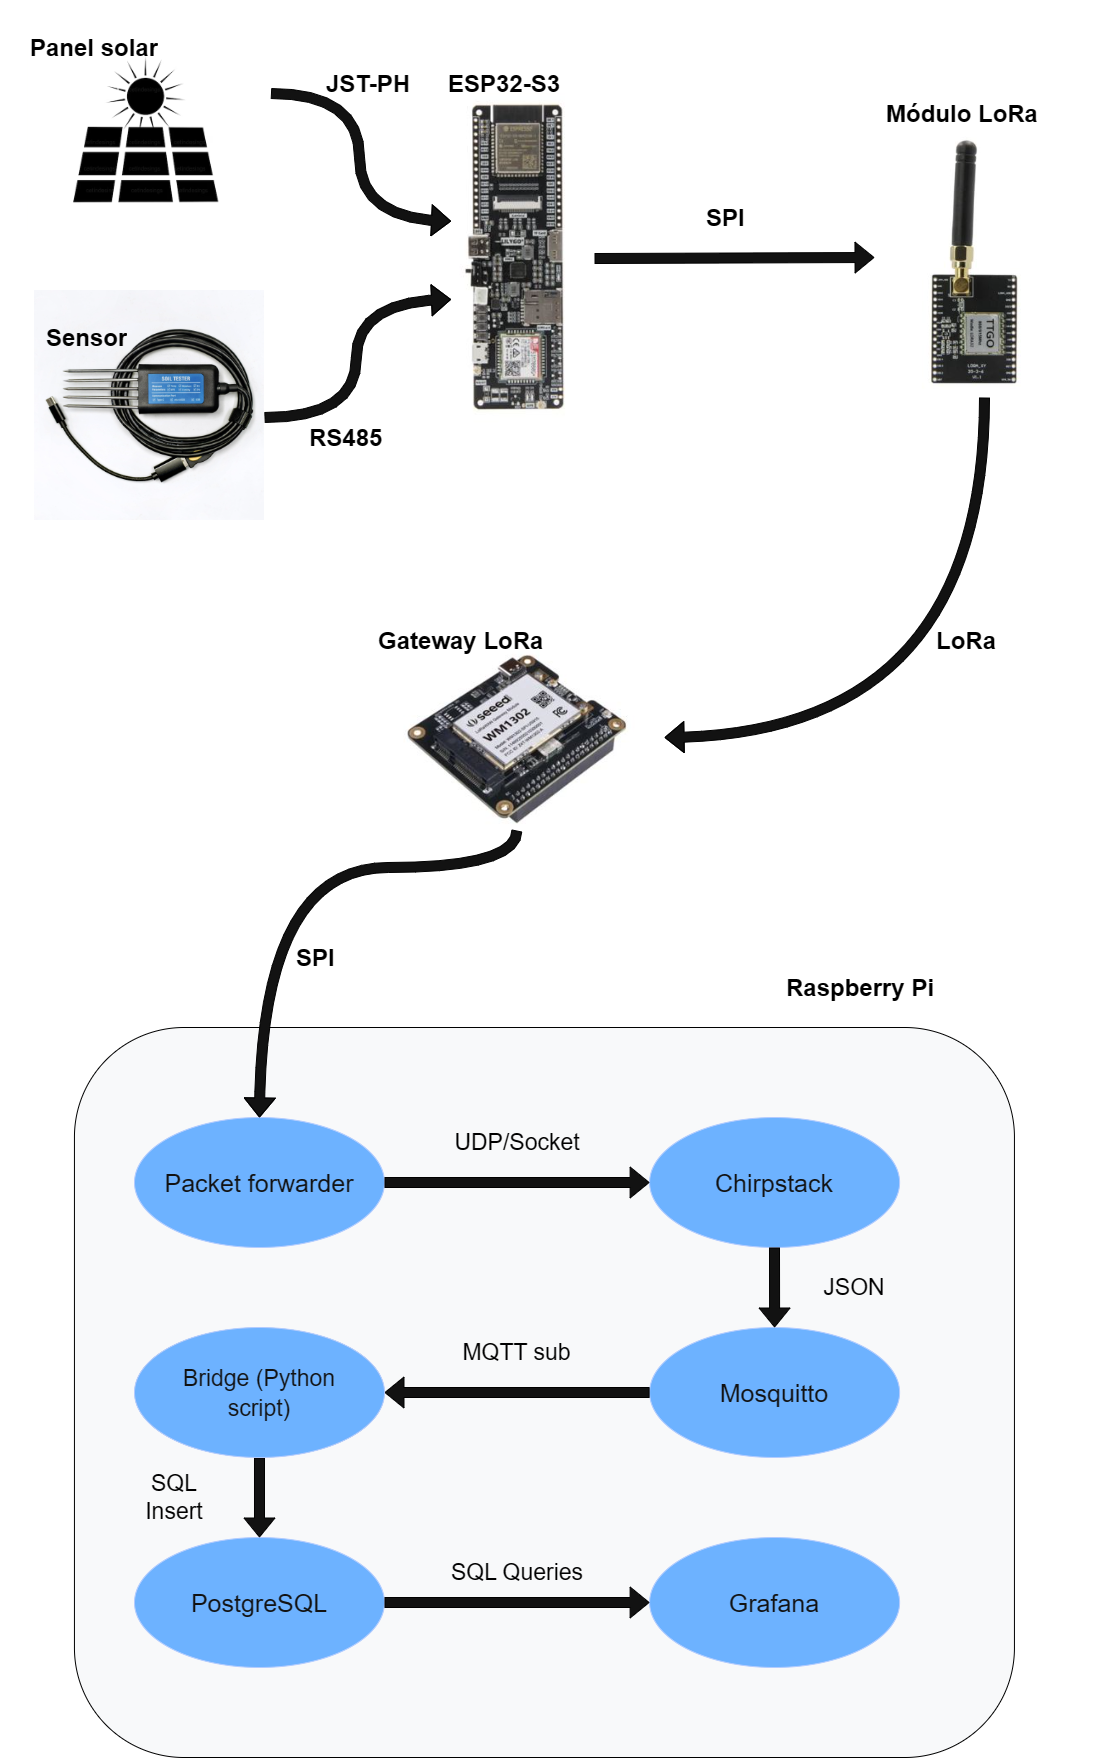
\includegraphics[width=0.72\textwidth]{figs/Diagrama.png}
    \caption{Arquitectura general del sistema extremo a extremo...}
    \label{fig:arquitectura_general}
\end{figure}

\subsection{Visión global y descomposición por capas}

La arquitectura se articula en una jerarquía modular estructurada en cinco capas funcionales diferenciadas:

\begin{enumerate}
    \item \textbf{Capa de percepción e instrumentación de campo:} Compuesta por una sonda industrial multivariable capaz de medir hasta 8 parámetros del sustrato (humedad volumétrica, temperatura, pH, conductividad eléctrica y nutrientes NPK). La comunicación física se canaliza mediante un bus serie industrial diferencial RS-485 inmune al ruido electromagnético, empleando el protocolo maestro-esclavo Modbus RTU para interrogar los registros del sensor bajo demanda.

    \item \textbf{Capa de computación embebida y control (Nodo sensor):} Gobernada por la placa LilyGO T-SIM7080G, provista de un microcontrolador ESP32-S3 de doble núcleo y una unidad de gestión de potencia (PMU AXP2101). Este nodo se encarga de orquestar el ciclo de vida energético del dispositivo, ejecutar la adquisición periódica, gestionar la sincronización horaria mediante el módem GNSS y salvaguardar los registros en memoria volátil retenida (\textit{RTC Slow RAM}) y tarjeta microSD antes de activar el transceptor de radio.

    \item \textbf{Capa de transporte inalámbrico LPWAN (Radio LoRa):} La comunicación de largo alcance se establece entre el módulo transceptor LoRa SX1276 conectado al microcontrolador mediante bus SPI y un concentrador multicanal SX1302 (\textit{Gateway} Seeed WM1302) alojado en la estación receptora. Las tramas se emiten bajo el estándar LoRaWAN en la banda libre europea EU868, empleando activación OTAA y mecanismos de transmisión agrupada por lotes (\textit{batching}) calculados dinámicamente según el factor de dispersión vigente.

    \item \textbf{Capa de pasarela y orquestación de red (Backend local):} Desplegada íntegramente sobre un miniordenador Raspberry Pi conectado físicamente por SPI al concentrador LoRa. La pasarela aloja:
    \begin{itemize}
        \item El demonio \textit{packet forwarder}, encargado de capturar las señales moduladas en el aire y transferirlas como paquetes UDP hacia el servidor de red.
        \item La pila del servidor LoRaWAN ChirpStack, que valida las claves de sesión criptográficas, controla los contadores de trama y ejecuta el decodificador JavaScript del perfil del dispositivo para desempaquetar la carga binaria útil.
        \item El intermediario de mensajería Eclipse Mosquitto (MQTT), que recibe los eventos de subida (\textit{uplink}) publicados por ChirpStack formateados en JSON estructurado.
    \end{itemize}

    \item \textbf{Capa de ingesta, persistencia relacional y analítica:} Un servicio residente en segundo plano programado en Python actúa como pasarela lógica (\textit{bridge}), suscribiéndose al intermediario MQTT, validando las cargas útiles e insertando las mediciones mediante sentencias SQL en un motor relacional PostgreSQL. Por último, la plataforma analítica Grafana consulta directamente las tablas indexadas de la base de datos para renderizar cuadros de mando interactivos y gráficos temporales en tiempo real.
\end{enumerate}

\subsection{Flujo de datos y ciclo de vida de la información}

El ciclo de vida del dato sigue una trazabilidad unidireccional y determinista diseñada para maximizar la integridad metrológica y minimizar el tiempo en el aire (\textit{airtime}) del enlace radio:

\begin{enumerate}
    \item \textbf{Muestreo e interrogación física:} Tras el despertar programado del microcontrolador desde el estado de suspensión profunda (\textit{Deep Sleep}), el PMU AXP2101 activa el carril de alimentación del transceptor RS-485. El ESP32-S3 emite una trama Modbus RTU de lectura (\texttt{Function Code 0x03}) hacia la sonda de suelo, recibiendo los registros binarios que contienen las magnitudes fisicoquímicas instantáneas.
    
    \item \textbf{Estructuración y persistencia de las muestras:} Los valores recibidos se empaquetan en una estructura binaria compacta (\texttt{struct Data} de 19 bytes) con la marca temporal del reloj del ESP32, sincronizado mediante GNSS cuando es posible. Las muestras se añaden a un búfer circular retenido en \textit{RTC Slow RAM}; esta retención no protege ante la pérdida completa de alimentación. La microSD mantiene un histórico JSON Lines (\texttt{.jsonl}), no una cola de reenvío. Solo al finalizar un conjunto por éxito local o segundo fallo se registra una entrada por muestra y se descarta ese conjunto. El excedente excluido del segundo intento por capacidad insuficiente queda para el lote siguiente, sin registro ni descarte anticipados. Si falla SD, se notifica y se descarta igualmente el conjunto finalizado.

    \item \textbf{Decisión de transmisión y conformación de trama:} Al alcanzar el umbral mínimo de cuatro muestras, el firmware enciende la radio y prepara la sesión para consultar la carga útil disponible. El primer envío espera un paquete completo; un lote pendiente se reintenta aunque no alcance la capacidad actual. Si falla la preparación antes de conocer esa capacidad, se seleccionan las cuatro muestras más antiguas. Tras el primer fallo, el estado retenido \texttt{pending\_batch} conserva la identidad, el tamaño y el intento consumido. En el segundo se intenta el prefijo que quepa, dejando el excedente para un lote nuevo; si no puede enviarse ninguna muestra, finaliza el lote pendiente completo. Un aplazamiento por ciclo de trabajo no consume intento ni modifica el conjunto pendiente. El éxito significa que la API de transmisión no devuelve error, sin acreditar recepción remota.

    \item \textbf{Recepción, demodulación y enrutado:} El concentrador Seeed WM1302 demodula la señal de radio en el extremo receptor y el \textit{packet forwarder} remite el paquete crudo mediante sockets UDP a ChirpStack. El servidor de red extrae la carga útil cifrada, autentica el dispositivo y ejecuta el decodificador JavaScript de la aplicación, convirtiendo el bloque binario en objetos JSON que se publican de forma inmediata en el \textit{broker} Mosquitto bajo el tópico correspondiente al dispositivo.

    \item \textbf{Ingesta, almacenamiento relacional y consulta:} El demonio de ingesta en Python, suscrito al \textit{broker} MQTT, consume los mensajes entrantes, desglosa los registros agrupados en muestras atómicas y ejecuta transacciones SQL (\texttt{INSERT}) en PostgreSQL. Los registros se asocian al identificador del nodo y a su marca de tiempo exacta (\texttt{TIMESTAMPTZ}). Grafana consulta de manera asíncrona la base de datos indexada, refrescando las series temporales de humedad, temperatura, electroconductividad y fertilidad NPK en el panel de supervisión.
\end{enumerate}

\subsection{Diagrama de despliegue}

El despliegue físico del sistema se divide en dos emplazamientos claramente diferenciados según sus requerimientos ambientales y energéticos:

\begin{itemize}
    \item \textbf{Emplazamiento de campo (Nodo sensor autónomo):}
    \begin{itemize}
        \item \textbf{Módulo de captación y acondicionamiento:} El sensor multivariable se encuentra enterrado en el perfil radicular del cultivo objetivo, conectado mediante un cable apantallado de par trenzado RS-485 hacia la envolvente del nodo.
        \item \textbf{Caja de control (IP67):} Contiene la placa base LilyGO T-SIM7080G (ESP32-S3), la tarjeta de expansión para el transceptor LoRa SX1276, el circuito transceptor RS-485 y la celda de batería recargable de litio.
        \item \textbf{Alimentación renovable:} Un panel solar fotovoltaico exterior acoplado mecánicamente al mástil se conecta mediante conector JST-PH directamente a la etapa de carga integrada y gobernada por el circuito PMU AXP2101, garantizando un funcionamiento energético autosuficiente y continuo.
    \end{itemize}

    \item \textbf{Infraestructura receptora y de servicios (Estación base):}
    \begin{itemize}
        \item \textbf{Pasarela física:} Formada por una Raspberry Pi montada en riel o encapsulado protector en las inmediaciones o caseta de la explotación, provista de alimentación continua y conectividad de red local.
        \item \textbf{Módulo concentrador LoRa:} La tarjeta Seeed WM1302 acoplada a la interfaz SPI de la Raspberry Pi y conectada a una antena omnidireccional de 868~MHz en el exterior para asegurar cobertura en línea de vista sobre la parcela sensorizada.
        \item \textbf{Entorno de ejecución de servicios:} La Raspberry Pi ejecuta un sistema operativo Linux donde coexisten y se autoinician bajo el gestor de demonios \texttt{systemd} los servicios del \textit{packet forwarder}, ChirpStack, Eclipse Mosquitto, el puente de ingesta en Python, PostgreSQL y el servidor Grafana accesible a través de navegador web en la red local.
    \end{itemize}
\end{itemize}

\section{Diseño hardware del nodo sensor}

En esta sección se detalla la composición física y electrónica del nodo sensor de campo. El enfoque de diseño adoptado combina la integración de módulos comerciales consolidados con el desarrollo de una placa portadora a medida (\textit{Carrier HAT}), reduciendo la complejidad de montaje, eliminando cableados volantes propensos a desconexiones y garantizando la robustez mecánica y eléctrica del dispositivo en campo.

\subsection{Composición e integración de subsistemas}
El diseño hardware parte de una arquitectura modular basada en componentes comerciales de amplia disponibilidad:

\begin{itemize}
    \item \textbf{Módulo de procesamiento y soporte base (LilyGO T-SIM7080G-S3):} Constituye el núcleo computacional del dispositivo. Esta placa integra en un único factor de forma compacto:
    \begin{itemize}
        \item El SoC \textbf{ESP32-S3} (doble núcleo Xtensa LX7), encargado de ejecutar el firmware, gestionar los ciclos de suspensión profunda (\textit{Deep Sleep}) y retener los datos en su memoria interna \texttt{RTC Slow RAM}.
        \item La unidad de gestión de potencia (\textbf{PMU AXP2101}), accesible por bus \text{I\textsuperscript{2}C}, que gobierna la carga de la batería LiPo de 3,7~V, admite entrada directa de panel solar fotovoltaico y permite habilitar o cortar la alimentación de los periféricos.
        \item El módem \textbf{SIM7080G}, del cual se explota exclusivamente su receptor GNSS integrado vía comandos AT sobre UART para calibrar periódicamente la deriva temporal (\textit{drift}) del oscilador RTC.
        \item El zócalo para tarjetas \textbf{microSD}, enlazado al controlador de bajo consumo SD-MMC en modo de 1 bit.
    \end{itemize}
    \item \textbf{Módulo transceptor LoRa (Semtech SX1276):} Módulo de comunicaciones inalámbricas de largo alcance que opera en la banda ISM EU868 (868,1--868,5~MHz). Se comunica con el microcontrolador mediante un bus serie SPI dedicado de cuatro hilos, acompañado de líneas de control y señalización de interrupciones (\texttt{DIO0}, \texttt{DIO1} y \texttt{RST}).
    \item \textbf{Sonda edafológica multivariable de campo:} Instrumento de sensado industrial enterrable que captura las variables fisicoquímicas del terreno (humedad, temperatura, conductividad, pH y macronutrientes NPK). Se comunica mediante par diferencial RS-485 bajo el protocolo Modbus RTU y precisa una tensión continua de alimentación en el rango de 9~V a 12~V.
\end{itemize}

\subsection{Placa de interconexión y acondicionamiento (Carrier HAT)}
Para articular de forma limpia la interconexión entre la placa LilyGO, el transceptor LoRa, la sonda de campo y las fuentes de energía, se diseñó y fabricó una placa portadora (\textit{carrier HAT}) a medida utilizando el entorno \textbf{KiCad EDA v7}.

En la Figura~\ref{fig:esquema_electrico} se presenta el esquema electrónico del circuito desarrollado, el cual aborda la adaptación de señales y la distribución de potencia necesaria para la sonda.

\begin{figure}[htbp]
    \centering
    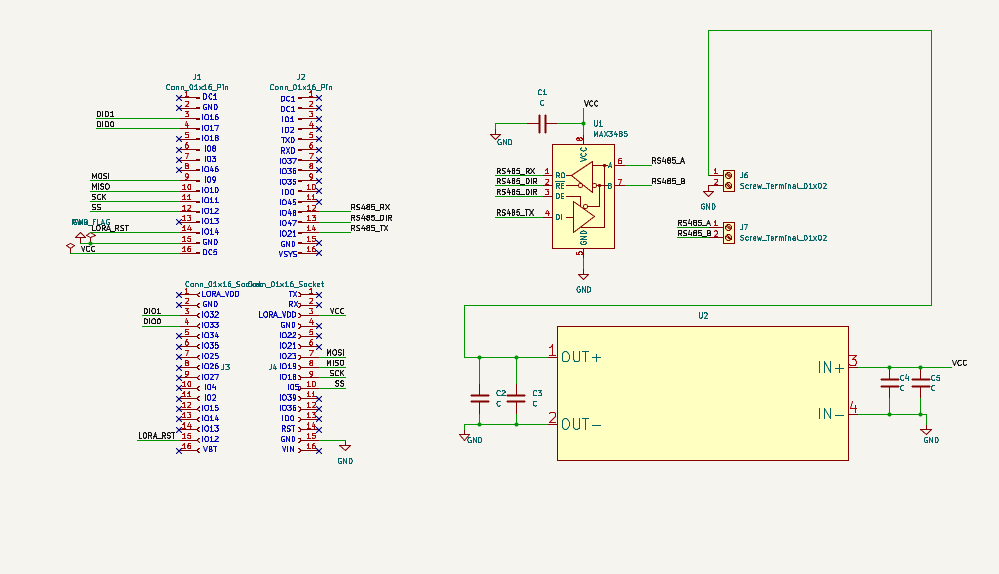
\includegraphics[width=0.95\textwidth]{figs/esquema_electrico.png}
    \caption{Esquema eléctrico del circuito del nodo sensor diseñado en KiCad.}
    \label{fig:esquema_electrico}
\end{figure}

El circuito esquemático resuelve los siguientes aspectos clave:
\begin{itemize}
    \item \textbf{Acondicionamiento y conversión a RS-485 (U1 - MAX3485):} Dado que el microcontrolador opera con niveles lógicos UART TTL a 3,3~V, se implementa el circuito integrado MAX3485 en encapsulado DIP-8 para convertir dichas señales al par diferencial del estándar RS-485. 
    \begin{itemize}
        \item La línea de recepción \texttt{RO} (pin 1) se mapea al pin \texttt{IO46} (\texttt{RS485\_RX}) y la de transmisión \texttt{DI} (pin 4) al pin \texttt{IO21} (\texttt{RS485\_TX}).
        \item Al ser una comunicación semidúplex, los pines de control de recepción ($\overline{\text{RE}}$, activo a nivel bajo) y transmisión ($\text{DE}$, activo a nivel alto) se puentean y quedan gobernados por una única línea de control: \texttt{RS485\_DIR}, conectada al pin \texttt{IO48} del ESP32-S3.
        \item La alimentación \texttt{VCC} del integrado se desacopla mediante el condensador cerámico $C_1$.
    \end{itemize}
    \item \textbf{Elevación de tensión para la sonda (U2 - Step-Up):} Debido a que la tensión nominal de la batería (3,7~V) es insuficiente para excitar la circuitería interna de la sonda NPK, se integra un módulo elevador DC-DC (U2). Su entrada \texttt{IN+} toma el carril \texttt{VCC} desacoplado por los condensadores $C_2$ y $C_3$, entregando por su salida \texttt{OUT+} una tensión regulada adecuada (filtrada por $C_4$ y $C_5$) hacia la borna de alimentación de la sonda.
    \item \textbf{Bornas de conexión de campo (\texttt{J6} y \texttt{J7}):} Terminales de tornillo verdes de dos polos para cableado hacia el exterior. La clema \texttt{J6} suministra la alimentación elevada (\texttt{OUT+}) y la masa (\texttt{GND}) hacia la sonda, mientras que la clema \texttt{J7} conecta el bus diferencial de datos (\texttt{RS485\_A} y \texttt{RS485\_B}).
\end{itemize}

\subsubsection{Mecanismo de acoplamiento físico y apilamiento (Stacking)}
La placa portadora actúa como nexo físico entre los diferentes módulos electrónicos mediante una estructura de apilamiento vertical que optimiza el espacio y prescinde por completo de cables de interconexión. En las Figuras~\ref{fig:pcb_render_top} y~\ref{fig:pcb_render_bottom} se ilustran, respectivamente, la cara superior y la cara inferior de la PCB diseñada:

\begin{figure}[htbp]
    \centering
    \begin{minipage}[t]{0.48\textwidth}
        \centering
        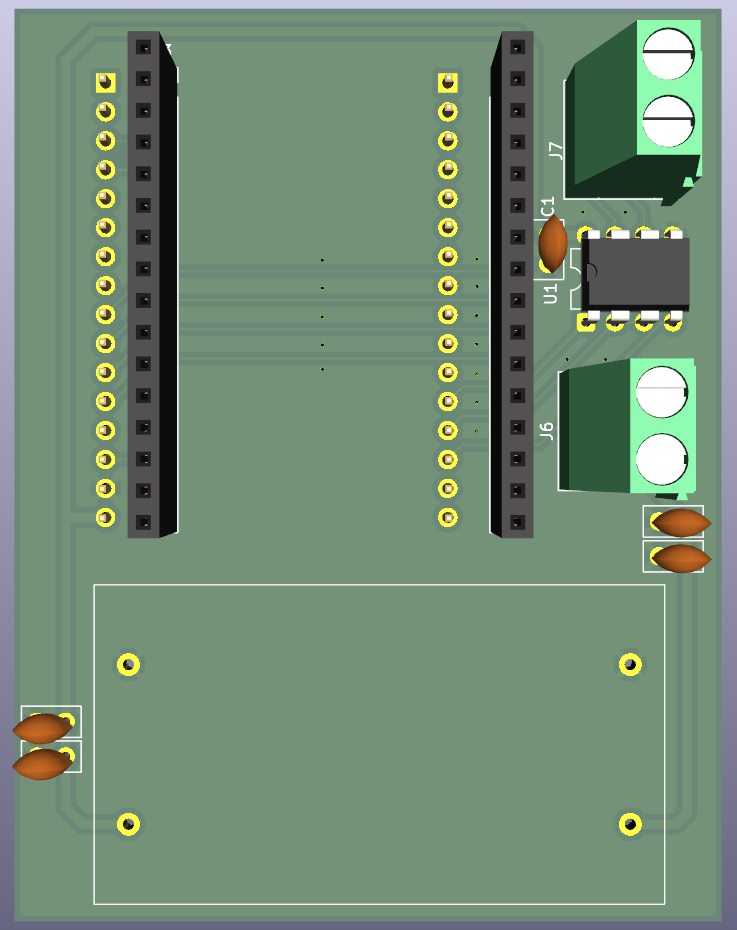
\includegraphics[width=\textwidth]{figs/pcb.png}
        \caption{Cara superior de la PCB: zócalos hembra para LoRa, integrado MAX3485, clemas y filtrado.}
        \label{fig:pcb_render_top}
    \end{minipage}
    \hfill
    \begin{minipage}[t]{0.48\textwidth}
        \centering
        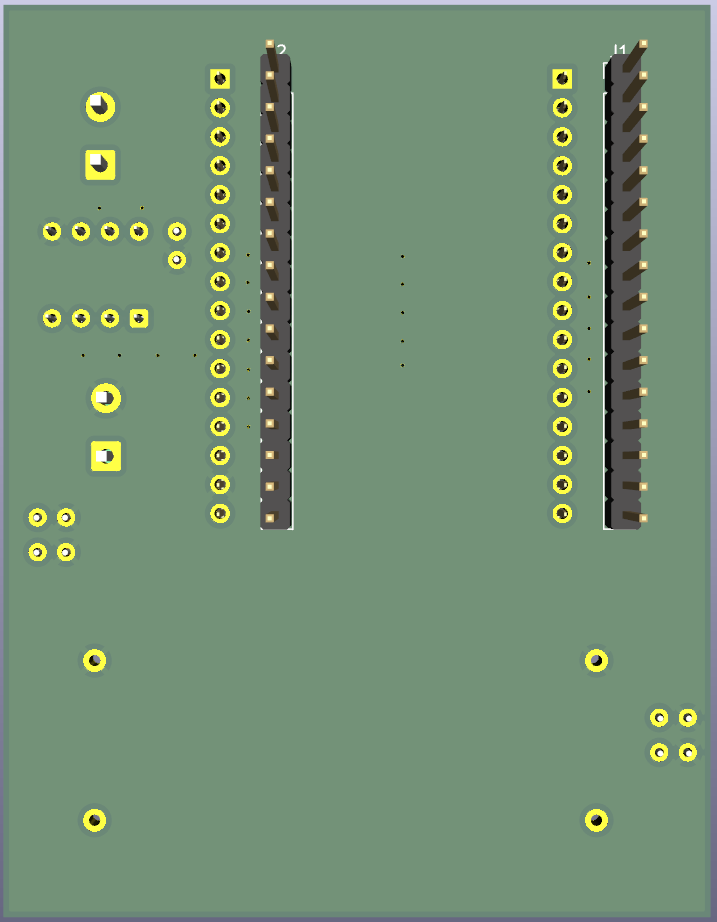
\includegraphics[width=\textwidth]{figs/pcb_bottom.png}
        \caption{Cara inferior de la PCB: tiras de pines macho (J1 y J2) para el acoplamiento directo a la LilyGO.}
        \label{fig:pcb_render_bottom}
    \end{minipage}
\end{figure}

El conexionado modular se fundamenta en las siguientes interfaces:
\begin{itemize}
    \item \textbf{Conexión del HAT a la placa LilyGO (Cara inferior):} En la cara inferior de la PCB se montan dos tiras de pines macho (\texttt{J1} y \texttt{J2}), tal como se aprecia en la Figura~\ref{fig:pcb_render_bottom}. Estas tiras encajan directamente sobre los conectores hembra de la placa LilyGO T-SIM7080G-S3 situada en la base, estableciendo el puente de alimentación (\texttt{VCC}, \texttt{GND}), las líneas de control serie para el MAX3485 y el bus SPI.
    \item \textbf{Conexión del módulo LoRa al HAT (Cara superior):} En la cara superior de la PCB se disponen dos tiras de pines hembra (\texttt{J3} y \texttt{J4}), visibles en la Figura~\ref{fig:pcb_render_top}. Sobre estos conectores hembra se pincha directamente el módulo transceptor LoRa SX1276, recibiendo la alimentación \texttt{VCC} y las líneas SPI y de control procedentes de la placa base a través de pistas dedicadas en la PCB.
    \item \textbf{Alojamiento de la etapa de potencia y filtrado:} En la cara superior se ubica el integrado MAX3485 (U1), los condensadores de desacoplo cerámicos y la huella serigrafiada con cuatro taladros de fijación para soldar el módulo elevador DC-DC (U2), manteniéndolo físicamente próximo a la clema de salida de alimentación (J6).
\end{itemize}

Este diseño de doble apilamiento (\textit{sandwich}) asegura que todo el conjunto quede ensamblado de forma compacta y rígida, facilitando su inserción en la caja estanca con certificación IP67.
% \begin{figure}[htbp]
%     \centering
%     \includegraphics[width=0.85\textwidth]{figuras/bloques_hardware.pdf}
%     \caption{Diagrama de bloques de la arquitectura hardware del nodo sensor.}
%     \label{fig:bloques_hardware}
% \end{figure}

\subsection{Etapa de alimentación y gestión de potencia}
Para asegurar una autonomía operativa indefinida sin recurrir a tendido eléctrico ni sustitución manual de baterías, el esquema de alimentación se apoya en un sistema de recolección fotovoltaica:

\begin{itemize}
    \item \textbf{Almacenamiento químico e interfaz solar:} El nodo integra una celda de polímero de litio (LiPo) de 3,7~V (2000~mAh) y una entrada para panel solar fotovoltaico exterior (rango de 4,4~V a 6,0~V), conectada a través de terminales JST-PH directamente a la etapa de carga lineal CC/CV del PMU AXP2101.
    \item \textbf{Monitoreo y protección ante sobredescarga:} Antes de iniciar los periféricos, el firmware consulta el porcentaje de batería que reporta la PMU. Si el valor es válido y está por debajo de \texttt{CRITICAL\_LEVEL} (10\,\%), el ciclo se aborta y el nodo vuelve a suspensión profunda. El firmware actual no comprueba aquí un umbral de tensión de 3,4~V.
    \item \textbf{Conmutación de carriles de potencia (\textit{Power Gating}):} Durante los intervalos de suspensión profunda (\textit{Deep Sleep}), el microcontrolador instruye al AXP2101 para que deshabilite los carriles LDO y DC-DC asociados a los elementos de mayor consumo (radio LoRa, módem y tarjeta SD). La memoria \texttt{RTC Slow RAM} conserva las lecturas en tránsito y el estado de sesión mientras el dominio RTC permanezca alimentado; esta retención no es persistente ante una pérdida completa de alimentación.
\end{itemize}

\subsection{Acondicionamiento del bus de campo RS-485}
La integración de la sonda industrial edafológica multivariable requiere adaptar los niveles lógicos del procesador a una línea diferencial semidúplex y suministrar la tensión de excitación adecuada:

\begin{itemize}
    \item \textbf{Transceptor diferencial (U1 - MAX3485):} Se implementa un circuito integrado MAX3485 en encapsulado DIP-8 alimentado por el carril de 3,3~V (\texttt{VCC}) y desacoplado localmente mediante el condensador cerámico de lenteja $C_1$. Su pin de recepción \texttt{RO} (pin 1) se conecta a la línea \texttt{RS485\_RX} (\texttt{IO46}) del microcontrolador, mientras que el pin de entrada de transmisión \texttt{DI} (pin 4) se conecta a la línea \texttt{RS485\_TX} (\texttt{IO21}).
    \item \textbf{Control del flujo de datos (\textit{Direction Control}):} Para operar en modo semidúplex sobre el par trenzado, los pines de habilitación de recepción ($\overline{\text{RE}}$, pin 2, activo a nivel bajo) y de transmisión ($\text{DE}$, pin 3, activo a nivel alto) se encuentran puenteados y gobernados por la línea de control \texttt{RS485\_DIR}, conectada al pin \texttt{IO48} del microcontrolador. Un nivel lógico alto en \texttt{IO48} conmuta el transceptor a modo de emisión para lanzar la trama de petición Modbus RTU, mientras que un nivel bajo lo devuelve al modo de escucha para recibir la respuesta de la sonda.
    \item \textbf{Elevación de tensión para la sonda (U2):} La sonda multivariable precisa una tensión de alimentación continua de 9 a 12~V, incompatible con el nivel nominal de la batería. Para ello, se incorpora un módulo elevador DC-DC \textit{Step-Up} (U2). La entrada \texttt{IN+} (pin 1) se alimenta desde el carril \texttt{VCC}, desacoplada en paralelo por los condensadores $C_2$ y $C_3$, mientras que la salida regulada de alta tensión \texttt{OUT+} (pin 3) se filtra mediante el par capacitivo $C_4$ y $C_5$.
    \item \textbf{Bornas de conexión externa (J6 y J7):} La interconexión física hacia el exterior de la caja se realiza mediante dos clemas de tornillo de paso estándar:
    \begin{itemize}
        \item \textbf{Clema J6 (Alimentación de la sonda):} El terminal 1 conecta la tensión elevada \texttt{OUT+} procedente de U2 y el terminal 2 conecta el retorno al plano de masa común (\texttt{GND}).
        \item \textbf{Clema J7 (Bus diferencial de datos):} El terminal 1 conecta la línea diferencial no inversora \texttt{RS485\_A} (pin 6 de U1) y el terminal 2 conecta la línea inversora \texttt{RS485\_B} (pin 7 de U1).
    \end{itemize}
\end{itemize}

\subsection{Diseño y ruteo de la placa de circuito impreso (PCB)}
El diseño esquemático y el trazado de la placa de circuito impreso tipo \textit{carrier HAT} se llevaron a cabo utilizando el entorno \textbf{KiCad EDA v7}. La placa actúa como chasis de integración física, permitiendo el conexionado directo entre el módulo de control LilyGO, el transceptor de radio y los periféricos de potencia:

\begin{itemize}
    \item \textbf{Topología física y apilamiento (\textit{Stacking}):} En la Figura~\ref{fig:pcb_nodo_3d} se muestra el renderizado tridimensional de la PCB desarrollada. La placa aloja en su cara superior dos pares de tiras de pines hembra:
    \begin{itemize}
        \item Tiras externas (\texttt{J1} y \texttt{J2}): Alojan la placa LilyGO T-SIM7080G-S3, enrutando las señales de alimentación (\texttt{VCC}, \texttt{GND}), el bus de control RS-485 (\texttt{IO46}, \texttt{IO48}, \texttt{IO21}) y el bus SPI de comunicaciones.
        \item Tiras internas (\texttt{J3} y \texttt{J4}): Permiten pinchar el módulo transceptor LoRa SX1276 (\texttt{J\_LORA}), conectando directamente sus líneas SPI (\texttt{MOSI}, \texttt{MISO}, \texttt{SCK}, \texttt{SS}) y pines de señal (\texttt{DIO0}, \texttt{DIO1}, \texttt{LORA\_RST}).
    \end{itemize}
    \item \textbf{Emplazamiento de potencia y filtrado capacitivo:} En la mitad inferior de la PCB se reservó una huella con cuatro taladros pasantes metalizados para el montaje mecánico del módulo elevador DC-DC (U2). Inmediatamente adyacentes a las entradas y salidas de potencia se rutearon pares de condensadores de filtrado en paralelo ($C_2/C_3$ a la entrada de U2, y $C_4/C_5$ a la salida hacia la clema J6) para absorber picos transitorios y rizado de conmutación.
    \item \textbf{Estrategia de desacoplo y planos de masa:} Para evitar interferencias en el receptor LoRa y prevenir caídas de tensión bruscas durante las ráfagas de transmisión de RF, se empleó una PCB de doble capa con un plano inferior de masa (\texttt{GND}) continuo. Se mantuvo una separación física deliberada entre la zona de conmutación de potencia (U2 y J6) y la zona digital/RF (MAX3485, conectores SPI de radio y bus de datos J7), reduciendo bucles de retorno y garantizando una alta relación señal/ruido en las lecturas analógicas y diferenciales.
\end{itemize}

% \begin{figure}[htbp]
%     \centering
%     \includegraphics[width=0.6\textwidth]{figuras/pcb_render_3d.png}
%     \caption{Renderizado tridimensional de la PCB HAT del nodo sensor diseñada en KiCad EDA.}
%     \label{fig:pcb_nodo_3d}
% \end{figure}

\section{Diseño del software embebido (Firmware)}

El firmware del nodo sensor ha sido desarrollado en lenguaje C++ utilizando un enfoque orientado a objetos, encapsulando las funcionalidades del hardware en módulos estáticos independientes (\texttt{Power}, \texttt{Clock}, \texttt{Lora}, \texttt{Modem}, \texttt{Sensor} y \texttt{SD}). El diseño lógico prioriza la eficiencia energética, la retención de datos en memoria no volátil y la optimización del tiempo de uso del espectro radioeléctrico.

\subsection{Ciclo de vida y máquina de estados del nodo}
La arquitectura de ejecución del nodo prescinde del tradicional bucle continuo (\texttt{loop()}) a favor de una máquina de estados lineal ejecutada íntegramente dentro de la rutina de inicialización \texttt{setup()}. Este paradigma garantiza que el microcontrolador permanezca activo estrictamente el tiempo necesario antes de transicionar al estado de suspensión profunda (\textit{Deep Sleep}):

\begin{itemize}
    \item \textbf{Arranque y evaluación energética:} Al despertar, el sistema habilita el hardware mínimo y evalúa el porcentaje de batería mediante la unidad de gestión de potencia (\texttt{PMU}). Si el nivel energético es inferior al umbral crítico (\texttt{CRITICAL\_LEVEL}), el nodo aborta la ejecución y vuelve a dormir para proteger la integridad química de la celda de litio.
    \item \textbf{Sincronización y adquisición:} Se inicializa un búfer circular en memoria retenida (\texttt{rtc\_buffer}) y se evalúa si el sistema requiere sincronización horaria absoluta (arranque en frío o si ha transcurrido más de un día desde la última calibración). A continuación, se captura el porcentaje de batería y la marca de tiempo, se energiza la sonda de campo, se realiza la lectura y se apaga inmediatamente la instrumentación para ahorrar energía.
    \item \textbf{Transición a reposo profundo:} Tras evaluar las condiciones de transmisión y persistir los datos, el nodo invoca la rutina \texttt{Power::enterDeepSleep()}. Esta función desconecta por hardware los reguladores del módem, la tarjeta SD y los periféricos de 3,3~V (carriles DC3, BLDO2, ALDO3 y DC5) y reinicia los pines de control pertinentes. El intervalo nominal es de 600\,s (10 minutos), definido por \texttt{DEEP\_SLEEP\_TIME\_S}; la expresión correspondiente es \texttt{600 * 1000000ULL} microsegundos. El tiempo activo se añade a la suspensión, por lo que no se trata de un periodo exacto de adquisición de 600\,s.
\end{itemize}

\subsection{Adquisición de campo y sincronización temporal}
Para garantizar la precisión de las series temporales y la integridad de las mediciones, el firmware integra rutinas específicas de interrogación industrial y calibración satelital:

\begin{itemize}
    \item \textbf{Interrogación Modbus RTU:} La captura de datos edafológicos se encapsula en la clase \texttt{Sensor}. Se excita el pin de control de dirección (\texttt{RS485\_DIR1}) y se transmite una trama de petición (\texttt{0x01, 0x03, 0x00, 0x00, 0x00, 0x07, 0x04, 0x08}) correspondiente a la lectura de registros de retención (\textit{Holding Registers}). El sistema queda a la escucha esperando una trama binaria de respuesta de 19 bytes que contiene las variables empaquetadas, retornando un estado de error si se excede el temporizador \texttt{SENSOR\_READ\_TIMEOUT}.
    \item \textbf{Sincronización horaria absoluta GNSS:} A través de la clase \texttt{Clock}, el nodo intenta corregir la deriva de su reloj de tiempo real (RTC) consultando al módem SIM7080G. La búsqueda de un \textit{fix} dispone de un máximo de 300\,s, al que se suman los tiempos de arranque y apagado del módem. De la respuesta \texttt{AT+CGNSINF} se comprueban el estado de \textit{fix} y el formato de fecha; la conversión fija explícitamente el huso UTC y rechaza fechas que se normalicen a otro día. La marca se aplica mediante \texttt{settimeofday}, comprobando su resultado, y \texttt{last\_sync\_timestamp} conserva la fecha del último éxito en RTC. La sincronización vuelve a vencer a las 24 horas (\texttt{SECONDS\_DAY = 86400}); los fallos se reintentan tras al menos 600\,s desde su finalización. Si no se obtiene hora válida, el muestreo, el envío y el registro continúan con el reloj del ESP32, sin garantizar UTC real hasta una sincronización posterior. No se corrigen retrospectivamente las marcas de las muestras ya adquiridas.
\end{itemize}

\subsection{Estructura de datos y persistencia multinivel}
El manejo de los datos muestreados se ha diseñado para minimizar los ciclos de escritura en almacenamiento no volátil y agilizar el empaquetado binario:

\begin{itemize}
    \item \textbf{Retención volátil de ultrabajo consumo:} Las muestras se encolan inicialmente en un búfer circular (\texttt{rtc\_buffer}) declarado con el atributo \texttt{RTC\_DATA\_ATTR}, lo que ubica esta estructura en la memoria \texttt{RTC Slow RAM} del microcontrolador. Esto permite acumular lecturas de forma continua durante los periodos de \textit{Deep Sleep} sin penalización de tiempo ni desgaste mecánico.
    \item \textbf{Validación del contexto retenido:} La firma \texttt{RTC\_BUFFER\_MAGIC = 0x52544247u} identifica el contexto del búfer y del lote pendiente. Si no coincide al arrancar, se reinician ambos y el contador de cabecera. La firma permite descartar un contexto incompatible, pero no comprueba por sí sola la integridad de todas las muestras ni recupera datos tras pérdida completa de alimentación.
    \item \textbf{Auditoría y persistencia local:} Cada conjunto finalizado se registra mediante una línea JSON por muestra en el archivo de la fecha del reloj del ESP32 al escribir, conservando las marcas originales. Tras éxito local o segundo fallo se descarta solo ese conjunto; el excedente reservado para el lote siguiente permanece en RTC. Si falla SD, se notifica y se descarta igualmente el conjunto finalizado. No se reenvía desde SD. No se garantiza atomicidad entre la escritura y la actualización de RTC si se interrumpe la alimentación durante la finalización.
\end{itemize}

\subsection{Estrategia de transmisión por lotes (Batching) y sesión LoRaWAN}
El subsistema de radio, gobernado por la clase \texttt{Lora}, implementa mecanismos avanzados para optimizar el tiempo de emisión en el aire (\textit{Airtime}) y acatar las normativas europeas sobre el ciclo de trabajo:

\begin{itemize}
    \item \textbf{Agrupación dinámica de lecturas (\textit{Batching}):} La capacidad se calcula mediante \texttt{node.getMaxPayloadLen() / sizeof(Data)} e incluye las restricciones del estado MAC y del \textit{Data Rate}. La primera transmisión requiere un lote completo según esa capacidad. La función \texttt{sendBatch()} recibe además un límite de muestras, para no incorporar al reintento las nuevas lecturas acumuladas.
    \item \textbf{Identidad y reintentos de envío:} \texttt{pending\_batch} retiene en RTC la referencia de la primera muestra, su conteo y los intentos consumidos. La referencia procede de \texttt{rtc\_buffer\_front\_id}, que avanza únicamente al descartar muestras de cabecera; no depende del timestamp. Un fallo de preparación de radio o sesión consume intento; \texttt{RADIOLIB\_ERR\_UPLINK\_UNAVAILABLE} aplaza la operación sin consumirlo. Tras el primer fallo se conserva el lote. Si la capacidad baja en el segundo, se finaliza solo el prefijo intentado, por éxito o segundo fallo, y el excedente conserva sus datos para un lote nuevo con dos intentos propios. Por ejemplo, de ocho muestras pendientes, si caben cinco se finalizan esas cinco y se reservan tres. Si no cabe ninguna o vuelve a fallar la preparación, se finaliza el lote pendiente completo. La SD se invoca solo al finalizar, no tras el primer fallo.
    \item \textbf{Preservación de la sesión OTAA:} Para evitar costosas renegociaciones de red (procedimiento \textit{Join}) tras cada ciclo de \textit{Deep Sleep}, el estado completo de la pila LoRaWAN (variables de sesión \texttt{lorawanSession} y contadores criptográficos \texttt{lorawanNonces}) se exporta y retiene en la memoria \texttt{RTC\_DATA\_ATTR}. 
    \item \textbf{Tolerancia a fallos de energía prolongados:} Adicionalmente, los contadores de tramas (\texttt{nonces}) se guardan de forma permanente en la memoria Flash (NVS) mediante la librería \texttt{Preferences}, previniendo ataques de repetición y desincronizaciones graves con el servidor de red \texttt{ChirpStack} ante un agotamiento total de la celda de litio.
    % TODO: Contrastar si el DevNonce debe persistirse en NVS tras un Join OTAA exitoso y validar el comportamiento con un arranque en frío.
\end{itemize}


\section{Diseño de la infraestructura de red y comunicaciones}
\subsection{Topología LoRaWAN y parámetros de modulación}
% Configuración de la banda regional EU868, canales, anchos de banda y esquema de activación OTAA.
\subsection{Preservación de sesión de red entre ciclos de reposo}
% Almacenamiento de claves criptográficas (NwkSKey, AppSKey) y contadores (FCntUp) en memoria retenida.
\subsection{Diseño del protocolo de mensajería interna (MQTT)}
% Jerarquía de topics para publicación de telemetría y eventos de red en ChirpStack.

\section{Diseño del backend y almacenamiento}
\subsection{Arquitectura desacoplada de la estación receptora}
% Separación de roles: Packet Forwarder, ChirpStack v4, Eclipse Mosquitto y servicio puente de ingesta.
\subsection{Diseño del servicio de ingesta y transformación}
% Lógica del demonio en Python para suscripción MQTT, validación de carga y persistencia.
\subsection{Modelo relacional de datos}
% Modelo Entidad-Relación y esquema de base de datos en PostgreSQL.
\subsection{Estrategia de indexación y optimización de consultas temporales}
% Definición de índices B-Tree sobre (device_eui, recorded_at DESC) y tipos TIMESTAMPTZ.

\section{Diseño de la plataforma de visualización}
\subsection{Estructura de cuadros de mando en Grafana}
% Definición de métricas agronómicas: paneles de series temporales, diagramas NPK y salud del nodo.
\subsection{Diseño de consultas analíticas y alertas}
% Definición conceptual de las sentencias SQL de extracción y umbrales de alerta de batería baja.

\chapter{Implementación y pruebas}
% Contenidos del capítulo.
% Las secciones presentadas son orientativas y no representan
% necesariamente la organización que debe tener este capítulo.
\section{Implementación}


\section{Pruebas funcionales}


\section{Pruebas de rendimiento}


\section{Pruebas de usabilidad}

\chapter{Conclusiones}
% Contenidos del capítulo.
% Las secciones presentadas son orientativas y no representan
% necesariamente la organización que debe tener este capítulo.

\section{Revisión de costes}

\section{Conclusiones}

\section{Trabajo futuro}




\pagestyle{appendix}

\appendix
\chapter{Apéndice}
\section{Ejemplos del lenguaje de marcado Latex}

Ths document is an example of BibTeX using in bibliography management. Three items 
are cited: \textit{The \LaTeX\ Companion} book \cite{latexcompanion}, the Einstein
journal paper \cite{einstein}, and the Donald Knuth's website \cite{knuthwebsite}. 
The \LaTeX\ related items are \cite{latexcompanion,knuthwebsite}\footnote{Esto está tomado de
\url{https://www.overleaf.com/learn/latex/Bibliography_management_with_bibtex}}.
 

  \textbf{Texto} en el párrafo 1.

  \textit{Texto} en el párrafo 2.

  \texttt{Texto} en el párrafo 3.


  \begin{itemize}
  \item Consideración 1
  \item Consideración 2
  \end{itemize}

  % Espacio vertical
  \vspace{0.5cm}
  
  \begin{enumerate}
  \item Punto 1
  \item Punto 2
  \end{enumerate}
  
A continuación se muestra una ecuación:

  \[ \int_{0}^{1}\frac{1}{x^2+1} dx \]

  Podemos incluir imágenes en formato: png, pdf o jpg.

  En la figura~\ref{fig:diagrama} se muestra un diagrama realizado con \href{yed}{https://www.yworks.com/products/yed}:

  \begin{figure}[!htb]
    \includegraphics[width=0.8\textwidth]{diagrama.pdf}
    \caption{Esta es una figura que latex decide donde colocar (floating) en el documento.}
    \label{fig:diagrama}
    \end{figure}

  \begin{tabular}{cc}
    Imagen 1 & Imagen 2 \\[2mm]
    \includegraphics[width=0.4\textwidth]{diagrama.pdf} &  \includegraphics[width=0.4\textwidth]{diagrama.pdf}
  \end{tabular}
  
  Este es un ejemplo de una tabla:
  
  \begin{tabular}{|l|c|}
    \hline
    Columna 1 & Columna 2 \\ \hline
    1 & 2 \\ \hline
  \end{tabular}


  \vspace*{1cm}
  O la misma tabla centrada:

  \begin{center}
    \begin{tabular}{|l|c|}
      \hline
      Columna 1 & Columna 2 \\ \hline
      1 & 2 \\ \hline
    \end{tabular}
  \end{center}

  Para generar el fichero PDF:
  
  \begin{lstlisting}{language=bash}
    pdflatex ejemplo-memoria.tex
    bibtex ejemplo-memoria
    pdflatex ejemplo-memoria.tex
\end{lstlisting}

  También se puede usar \texttt{latexmk} que automáticamente regenera la bibliografía.
  \begin{lstlisting}{language=bash}
    latexmk -pdf ejemplo-memoria.tex
\end{lstlisting}

  


\addcontentsline{toc}{chapter}{Bibliografía}
\bibliographystyle{unsrt}
\bibliography{bib/bibliografia}




\end{document}

%%% Local Variables:
%%% mode: latex
%%% TeX-master: t
%%% End:
